\chapter{随机与分块优化}
\label{chap:opt-stochastic-block}

设最小二乘目标由一百万行数据构成，每一行贡献一项$\tfrac12(\bm a_i^\top\bm x-b_i)^2$。梯度下降每走一步都要把一百万行读一遍，可是任取一行，它给出的梯度$\bm a_i(\bm a_i^\top\bm x-b_i)$读取代价只有百万分之一，而且在随机取行的意义下“平均起来”恰好是完整梯度。用这样的读数代替完整梯度，单步方向可能偏得很远，甚至指向上坡；那么很多步合起来是否仍在下降，又会停在离最小点多远的地方？同样的问题也出现在变量一侧：参数有上亿个坐标时，我们可能只想每次更新其中一块，或者轮流固定一部分变量求解较小的子问题。

本章研究这三种节省：少读取目标项、复用历史读数、只更新部分变量。学习目标是说清每种节省在什么条件下仍给出可控的进展，进展用什么对象衡量，又付出了哪些额外代价。主线采用有限步的期望误差界：给定迭代次数，界住目标差、到最小点距离的平方或梯度范数平方的期望。它回答“平均而言跑$T$步能到哪里”，不回答“每条随机路径最终是否收敛”；后者需要鞅与随机逼近工具，归第~\ref{chap:stochastic-processes-and-approximation}章。

各节按被改变的计算对象相连。先固定被优化的目标和随机性来源，区分求解误差与统计误差；然后把随机读数接入梯度更新，用条件期望建立单步递推，由此得到常数步长的噪声邻域、递减步长的收敛速率以及返回点的选择。噪声邻域提示下一步要压低方向的波动：重新设计抽样、扩大批量，或者借助快照与梯度记忆把方差降到零。历史读数也可以用来调整尺度，这就是AdaGrad、Adam等逐坐标方法以及矩阵尺度方法。随后改变每轮更新的变量范围，研究坐标下降与交替最小化。实际读数还常被裁剪或替换，这需要回到原目标核查方向的含义。最后两节比较各种误差怎样进入轨迹、样本替换怎样影响输出，并把所有方法放在同一预算口径下比较。

\section{有限和与期望目标}
\label{sec:opt-sto-objectives}

随机算法里有两种随机性容易混在一起：数据本身是从某个总体中抽来的，算法每一步又随机挑选读取哪些数据。前者决定我们在优化哪个函数，后者只决定求解过程看到哪些信息。本节先把被优化的目标固定下来，说明一次完整梯度要付出什么代价，再把有限平均推广到期望，并指出微分与期望交换所需的条件。后面各节的分析都针对这里选定的目标。

\subsection{固定样本的有限和}
\label{sec:opt-sto-finite-sum}

\paragraph{逐项平均的目标}
机器学习中的目标通常是逐样本损失的平均。给定$n$个样本，第$i$个样本贡献一个函数$f_i:\mathbb R^d\to\mathbb R$，目标是
\begin{equation}
\label{eq:opt-sto-finite-sum}
  f(\bm x)=\frac1n\sum_{i=1}^n f_i(\bm x).
\end{equation}
这种形式称为\term{有限和目标}（finite-sum objective）。正则项可以平均分摊到每一项里，也可以单独写出。本章的主要例子是岭回归形式的最小二乘：取$\bm A\in\mathbb R^{n\times d}$的第$i$行为$\bm a_i^\top$，
\[
  f_i(\bm x)=\tfrac12(\bm a_i^\top\bm x-b_i)^2+\tfrac{\lambda}{2}\lVert\bm x\rVert_2^2,\qquad
  f(\bm x)=\frac1{2n}\lVert\bm A\bm x-\bm b\rVert_2^2+\frac{\lambda}{2}\lVert\bm x\rVert_2^2 .
\]
它与本部分通用的写法$\tfrac12\lVert\bm A\bm x-\bm b\rVert_2^2+\tfrac{\lambda'}{2}\lVert\bm x\rVert_2^2$只差整体因子$1/n$和记号$\lambda'=n\lambda$，最小点相同。这里除以$n$，是为了让目标值和梯度的量级不随样本数增长，步长也就不必随$n$重新换算。

\paragraph{一次完整梯度的代价}
完整梯度$\nabla f(\bm x)=\frac1n\sum_i\nabla f_i(\bm x)$需要读取全部$n$项。对上面的最小二乘，$\nabla f_i(\bm x)=\bm a_i(\bm a_i^\top\bm x-b_i)+\lambda\bm x$，一项的计算量是$O(d)$，完整梯度是$O(nd)$。$n$达到百万、数据存放在磁盘或分布在多台机器上时，读一遍数据本身就是主要开销。相比之下，只读一项的代价与$n$无关。本章所说的“少读取”，指的就是用一部分项的梯度代替这$n$项的平均。

需要强调的是，数据一旦固定，$f$就是一个确定的函数，它的最小点、最优值和梯度都没有随机性。随机抽取下标只改变算法在某一步获得的信息：同一个点$\bm x$，抽到不同的项会读到不同的向量。后面说“随机梯度的期望等于梯度”，期望是对抽样下标取的，被比较的仍是这个确定目标的梯度。

\begin{example}[三点平均]
\label{ex:opt-sto-three-points}
取$d=1$、$n=3$，$f_i(x)=\tfrac12(x-c_i)^2$，$c_1=0$、$c_2=1$、$c_3=5$。目标
\[
  f(x)=\frac16\bigl(x^2+(x-1)^2+(x-5)^2\bigr)=\frac12(x-2)^2+\frac73
\]
在$x^\star=2$处取得最小值$f^\star=7/3$，它是$1$强凸、$1$光滑的。在$x=3$处，三项的梯度$x-c_i$分别是$3$、$2$、$-2$，平均为$1=f'(3)$。第三项的读数$-2$与真梯度符号相反：如果这一步只看它，就会向右走，离最小点更远。这个例子会在本章反复使用，因为每项曲率相同，许多量可以精确算出。
\end{example}

\paragraph{目标项分解与变量分块}
减少计算还有另一个方向。有限和把目标按\emph{项}拆开，读取其中一部分；变量分块则把$\bm x$按\emph{坐标}拆成若干块，每轮只更新其中一块，其余坐标保持不变。图~\ref{fig:opt-sto-sum-vs-block}把两者画在同一个数据矩阵上：前者选行，后者选列。两者互不排斥，例如可以抽一批样本、只更新这批样本涉及的那些坐标。但每种节省都改变了“一步”的含义，因此分析时必须记录每次调用的三样东西：在哪个点求值，按什么分布抽取了哪些项或哪些坐标，返回了什么向量。后文的收敛结论都依赖于这些记录满足的条件。

\begin{figure}[!htbp]
  \centering
  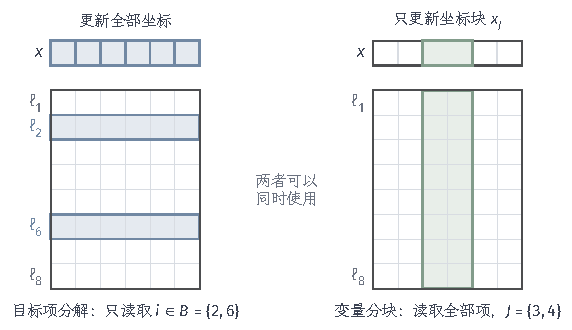
\includegraphics[width=96.855mm]{figures/03-optimization-evolution-and-signals/01-optimization/tikz/c6-sum-vs-block/figure.pdf}
  \caption{同一个数据矩阵上的两种节省。网格的$8$行对应$8$个目标项$\ell_i$，$6$列对应决策变量的$6$个坐标，顶部一行表示$\bm x$。左：目标项分解，本轮只读取第$2$、$6$行（蓝色），但所得方向更新全部坐标。右：变量分块，本轮读取全部行，只更新第$3$、$4$个坐标组成的块$\bm x_J$（绿色）。}
  \label{fig:opt-sto-sum-vs-block}
\end{figure}

\subsection{期望目标与随机梯度}
\label{sec:opt-sto-expectation}

\paragraph{从有限平均到期望}
有限和是一种特殊的期望：令下标$I$在$\{1,\dots,n\}$上均匀分布，就有$f(\bm x)=\mathbb E[f_I(\bm x)]$。更一般地，设$\xi$是取值于某个空间的随机变量，$f(\bm x;\xi)$是给定$\xi$时的损失，目标
\begin{equation}
\label{eq:opt-sto-expectation}
  F(\bm x)=\mathbb E_\xi\bigl[f(\bm x;\xi)\bigr]
\end{equation}
称为期望目标。按照能否获得$\xi$的分布，可以分三种情形。若分布已知且期望能算出闭式，$F$就是普通的确定目标。若只能从分布中采样，例如数据持续到来、每个样本只用一次，那么每次采样得到一个新的读数，算法直接面对$F$。若先收集$n$个样本$\xi_1,\dots,\xi_n$，再用$\frac1n\sum_if(\bm x;\xi_i)$代替$F$，就回到有限和~\eqref{eq:opt-sto-finite-sum}，这个平均在学习问题中称为\term{经验风险}（empirical risk），$F$则对应\term{期望风险}（expected risk）。

\paragraph{微分与期望何时可交换}
期望目标的随机梯度通常取为$\nabla_{\bm x}f(\bm x;\xi)$。要让它的期望等于$\nabla F(\bm x)$，需要把梯度移到期望里面。积分号下求导定理给出一个常用的充分条件：若在$\bm x$的某个邻域内，对几乎每个$\xi$，$f(\cdot;\xi)$可微，且偏导数被一个可积函数$G(\xi)$统一控制，$\lVert\nabla_{\bm x}f(\bm y;\xi)\rVert_2\leq G(\xi)$对邻域内所有$\bm y$成立，$\mathbb E[G(\xi)]<\infty$，同时$f(\bm x;\cdot)$本身可积，则$F$在$\bm x$可微且$\nabla F(\bm x)=\mathbb E[\nabla_{\bm x}f(\bm x;\xi)]$。该定理的证明基于中值定理与控制收敛定理，可参考\BookChapterRef{chap:integration}{卷二“积分”章}；这里只用它的结论。有限和情形下期望是有限加权和，只要每项可微，交换自动成立。

条件不满足时，交换可能失败，而且失败的方式很隐蔽。设$\xi$在$[0,1]$上均匀分布，$f(x;\xi)=\mathbb 1_{\{\xi\leq x\}}$。对$x\in(0,1)$，$F(x)=\mathbb P(\xi\leq x)=x$，导数为$1$。可是对每个固定的$\xi\neq x$，$f(\cdot;\xi)$在$x$附近是常数，逐样本导数为零，于是$\mathbb E[\partial_xf(x;\xi)]=0\neq1$。问题出在跳跃点$\xi$随样本移动：差商$(f(x+h;\xi)-f(x;\xi))/h$在一个概率为$h$的集合上等于$1/h$，无法被与$h$无关的可积函数控制。目标在平均意义下光滑，不代表逐样本的梯度可以拿来作无偏读数。第~\ref{sec:opt-sto-surrogate}节的离散前向会再遇到这种现象。

\paragraph{估计总体梯度与求解经验目标}
在学习问题里，人们最终关心的常是期望风险$F$，手里却只有固定的$n$个样本。这时存在两种不同的误差。其一来自数据：经验风险的最小点与期望风险的最小点不同，这个差距由样本量和模型决定，再精确地求解经验风险也消除不了。其二来自计算：在固定的经验风险上，算法跑了有限步，返回点与经验最小点之间还有差距。本章研究的是后一种：选定一个目标（有限和或期望），分析算法在有限步后能把这个目标的误差降到多少。经验最小点与总体最小点之间的差距、模型选择与泛化保证属于统计问题，由后续讨论学习理论的部分承担。两种误差可以相互权衡，例如数据有限时不必把优化误差压到远低于统计误差的水平，但它们的来源与控制手段不同，不能用同一个数字代表。

\section{随机梯度方法}
\label{sec:opt-sto-sgd}

上一节固定了目标，并看到单项读数可能指向上坡。本节把这样的读数直接代入梯度下降，研究“单步可能变坏、平均仍在变好”这件事怎样精确表述。工具是条件期望：给定到目前为止发生的一切，下一步读数的平均是什么。由此得到一条单步递推，后面的常数步长误差、递减步长速率和返回点的选择都从它推出。

\subsection{条件无偏与读数误差}
\label{sec:opt-sto-unbiased}

\paragraph{历史与条件期望}
随机算法的第$t$步发生之前，初值$\bm x^{(0)}$以及前$t$步抽到的下标$i^{(0)},\dots,i^{(t-1)}$都已经确定，迭代点$\bm x^{(t)}$是它们的函数。把这些已经观察到的随机量所含的信息记为\emph{历史}$\mathcal F^{(t)}$，严格地说，它是由这些随机量生成的$\sigma$代数。给定历史后的条件期望记作
\[
  \mathbb E_t[\,\cdot\,]=\mathbb E\bigl[\,\cdot\mid\mathcal F^{(t)}\bigr].
\]
本章只用条件期望的三条基本性质：由历史决定的量（如$\bm x^{(t)}$、$\nabla f(\bm x^{(t)})$）可以像常数一样提到$\mathbb E_t$外面；若新的下标$i^{(t)}$与历史独立，则$\mathbb E_t[\phi(\bm x^{(t)},i^{(t)})]$等于把$\bm x^{(t)}$当作固定点、只对$i^{(t)}$求平均；以及全期望公式$\mathbb E[\mathbb E_t[Z]]=\mathbb E[Z]$。这些性质的严格陈述和证明见\BookChapterRef{chap:conditional-expectation}{卷二“条件期望与条件分布”章}。

\paragraph{条件无偏的读数}
第$t$步算法得到一个向量$\bm g^{(t)}$，用来代替$\nabla f(\bm x^{(t)})$。我们需要的不是“平均来说$\bm g^{(t)}$与梯度差不多”，而是“站在当前点、看着已有的历史，下一次读数的平均正好是这里的梯度”。

\begin{definition}[条件无偏读数]
\label{def:opt-sto-unbiased}
设$\bm g^{(t)}$是可积随机向量。若
\[
  \mathbb E_t\bigl[\bm g^{(t)}\bigr]=\nabla f(\bm x^{(t)})
\]
几乎必然成立，称$\bm g^{(t)}$是$\nabla f$在$\bm x^{(t)}$处的\term{条件无偏}（conditionally unbiased）读数，也称\term{随机梯度}（stochastic gradient）。
\end{definition}

对有限和~\eqref{eq:opt-sto-finite-sum}，若$i^{(t)}$在$\{1,\dots,n\}$上均匀分布且与历史独立，则$\bm g^{(t)}=\nabla f_{i^{(t)}}(\bm x^{(t)})$满足$\mathbb E_t[\bm g^{(t)}]=\frac1n\sum_i\nabla f_i(\bm x^{(t)})=\nabla f(\bm x^{(t)})$，这正是上述第二条性质。条件版本比无条件的$\mathbb E[\bm g^{(t)}]=\mathbb E[\nabla f(\bm x^{(t)})]$强得多：如果抽样规则看了当前位置，例如在三点例中$x>2$时总抽第一项、$x<2$时总抽第三项，那么每一步的读数都系统性地偏离当地梯度，即使把所有时刻混在一起平均，偏差也可能互相抵消而看不出来。后面的单步分析在每个固定历史下取平均，所以需要的正是条件无偏。

\paragraph{读数的分解}
一般的读数未必无偏，例如被截断、量化或者用了过时的参数。把它拆成三部分：
\begin{equation}
\label{eq:opt-sto-reading-split}
\begin{aligned}
  \bm g^{(t)}&=\nabla f(\bm x^{(t)})+\bm\beta^{(t)}+\bm\xi^{(t)},\\
  \bm\beta^{(t)}&=\mathbb E_t[\bm g^{(t)}]-\nabla f(\bm x^{(t)}),\qquad
  \bm\xi^{(t)}=\bm g^{(t)}-\mathbb E_t[\bm g^{(t)}].
\end{aligned}
\end{equation}
$\bm\beta^{(t)}$是\emph{条件偏差}，由历史决定；$\bm\xi^{(t)}$是\emph{噪声}，满足$\mathbb E_t[\bm\xi^{(t)}]=\bm0$。两者需要分别控制，常用的假设是$\lVert\bm\beta^{(t)}\rVert_2\leq B$与$\mathbb E_t\lVert\bm\xi^{(t)}\rVert_2^2\leq\sigma^2$。条件无偏就是$\bm\beta^{(t)}=\bm0$。此时把$\lVert\bm g^{(t)}\rVert_2^2$展开，交叉项$2\langle\nabla f(\bm x^{(t)}),\bm\xi^{(t)}\rangle$的条件期望为零，得到后面反复使用的恒等式
\begin{equation}
\label{eq:opt-sto-second-moment}
  \mathbb E_t\lVert\bm g^{(t)}\rVert_2^2=\lVert\nabla f(\bm x^{(t)})\rVert_2^2+\mathbb E_t\lVert\bm\xi^{(t)}\rVert_2^2 .
\end{equation}
读数的平均平方长度等于真梯度的平方长度加上噪声的方差：噪声只会让读数变长，不会让它变短。

\paragraph{无偏不等于下降，也不等于方差小}
在三点例的$x=3$处，三个读数$3,2,-2$以等概率出现，平均为$1$。读数$-2$与真梯度方向相反，沿它走一步会上坡，这种情况的概率是$1/3$。噪声的方差为$\mathbb E_t(\xi^{(t)})^2=\frac13\bigl(2^2+1^2+3^2\bigr)=\frac{14}3$，远大于真梯度的平方$1$。由于每一项曲率相同，噪声$\xi^{(t)}=(x-c_{i^{(t)}})-(x-2)=2-c_{i^{(t)}}$与$x$无关，这个方差在任何点都是$14/3$；即使站在最小点$x^\star=2$，读数仍是$2,1,-3$之一，算法仍会被推离最小点。图~\ref{fig:opt-sto-gradient-fan}在二维最小二乘上画出同样的现象：十个逐项下降方向散成一把扇子，其中三个与平均方向成钝角，只有平均才指向等高线的内侧。

\begin{figure}[!htbp]
  \centering
  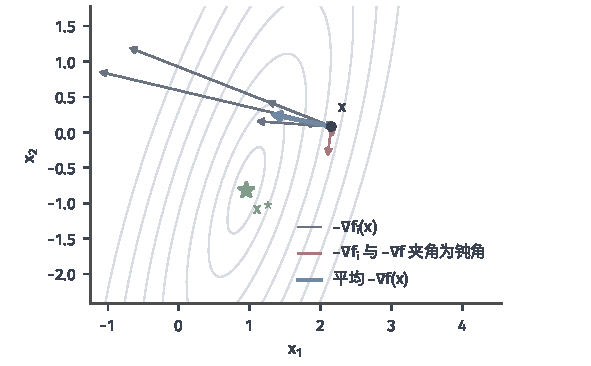
\includegraphics[width=100mm]{figures/03-optimization-evolution-and-signals/01-optimization/matplotlib/c6-gradient-fan/figure.pdf}
  \caption{一点处的逐项读数。目标是$n=10$、$d=2$的岭回归最小二乘，灰色曲线为等高线，星号为最小点。从黑点$\bm x$出发的细箭头是逐项下降方向$-\nabla f_i(\bm x)$（按$0.35$倍画出），其中红色的三个与平均方向夹角为钝角，单独沿它们走一小步会使目标上升；粗蓝箭头是它们的平均$-\nabla f(\bm x)$。数据由固定种子生成，参数见图源记录。}
  \label{fig:opt-sto-gradient-fan}
\end{figure}

\subsection{随机梯度下降与步长}
\label{sec:opt-sto-sgd-step}

\paragraph{一轮更新}
把读数代入梯度下降，就得到\term{随机梯度下降}（stochastic gradient descent）。下面的算法写清每一轮的四个动作：抽样、读取、更新和记录。步长$\eta^{(t)}$必须在抽取$i^{(t)}$之前确定，即由历史决定；否则步长与读数相关，条件期望就不能把它们分开处理。

\begin{algorithm}[随机梯度下降]
\label{alg:opt-sto-sgd}
\begin{algorithmic}[1]
\Require 初值$\bm x^{(0)}$，步长序列$\eta^{(0)},\eta^{(1)},\dots$（由历史决定），轮数$T$，抽样分布
\Ensure 返回点（最后一点、加权平均点或随机选出的迭代点，见第~\ref{sec:opt-sto-return}节）
\For{$t=0,1,\dots,T-1$}
  \State 与历史独立地抽取下标$i^{(t)}$
  \State 读取$\bm g^{(t)}=\nabla f_{i^{(t)}}(\bm x^{(t)})$
  \State $\bm x^{(t+1)}=\bm x^{(t)}-\eta^{(t)}\bm g^{(t)}$
  \State 按所选返回规则更新记录（如累加$\eta^{(t)}\bm x^{(t)}$）
\EndFor
\end{algorithmic}
\end{algorithm}

每轮读取一项，计算$O(d)$，额外存储只有返回规则所需的一个向量。每轮\emph{重新}抽样是关键。若始终使用同一个下标$i$，算法就是对$f_i$的普通梯度下降，收敛到$f_i$的最小点而不是$f$的最小点：在三点例中始终读第三项，迭代会走向$5$。重新抽样让不同项的偏向在多步中相互抵消。

\paragraph{代入光滑上界}
随机梯度的单步分析与梯度下降相同，只是在最后对新下标取条件期望。设$f$是$L$光滑的，第~\ref{chap:opt-smooth}章的下降引理给出$f(\bm x+\bm p)\leq f(\bm x)+\langle\nabla f(\bm x),\bm p\rangle+\tfrac L2\lVert\bm p\rVert_2^2$。

\begin{lemma}[随机梯度的单步下降]
\label{lem:opt-sto-one-step}
设$f$在$\mathbb R^d$上$L$光滑，$\bm g^{(t)}$条件无偏且$\mathbb E_t\lVert\bm g^{(t)}-\nabla f(\bm x^{(t)})\rVert_2^2\leq\sigma^2$，步长$\eta=\eta^{(t)}$由历史决定。则$\bm x^{(t+1)}=\bm x^{(t)}-\eta\bm g^{(t)}$满足
\begin{equation}
\label{eq:opt-sto-one-step}
  \mathbb E_t f(\bm x^{(t+1)})\leq f(\bm x^{(t)})-\eta\Bigl(1-\frac{L\eta}2\Bigr)\lVert\nabla f(\bm x^{(t)})\rVert_2^2+\frac{L\eta^2}{2}\sigma^2 .
\end{equation}
\end{lemma}

\begin{proof}
取$\bm p=-\eta\bm g^{(t)}$代入下降引理：
\[
  f(\bm x^{(t+1)})\leq f(\bm x^{(t)})-\eta\langle\nabla f(\bm x^{(t)}),\bm g^{(t)}\rangle+\tfrac{L\eta^2}2\lVert\bm g^{(t)}\rVert_2^2 .
\]
对两边取$\mathbb E_t$。$f(\bm x^{(t)})$、$\nabla f(\bm x^{(t)})$与$\eta$由历史决定，可以提出；由条件无偏，$\mathbb E_t\langle\nabla f(\bm x^{(t)}),\bm g^{(t)}\rangle=\lVert\nabla f(\bm x^{(t)})\rVert_2^2$；由式~\eqref{eq:opt-sto-second-moment}，$\mathbb E_t\lVert\bm g^{(t)}\rVert_2^2\leq\lVert\nabla f(\bm x^{(t)})\rVert_2^2+\sigma^2$。代入即得。
\end{proof}

与梯度下降相比，式~\eqref{eq:opt-sto-one-step}多出了最后一项$\tfrac{L\eta^2}2\sigma^2$。中间项是期望下降量，正比于$\eta$；最后一项是噪声造成的期望上升，正比于$\eta^2$。远离驻点时梯度大，下降项占优；接近驻点时梯度趋于零，噪声项不随之减小，单步不再保证期望下降。这就是随机梯度不能像梯度下降那样一直走到驻点的原因。

\paragraph{强凸目标的距离递推}
要说清误差停在哪里，用到最小点距离的平方更方便。对有限和，我们把方差假设换成一个在整个空间成立的条件：每项凸且光滑。最小二乘满足这个条件，而“读数方差处处不超过$\sigma^2$”对最小二乘只在有界区域内成立，因为$\nabla f_i(\bm x)-\nabla f(\bm x)$随$\lVert\bm x\rVert_2$线性增长。

先准备一个凸光滑函数的不等式。它说梯度的变化量可以被函数值相对于切平面的高度控制。

\begin{lemma}[凸光滑函数的梯度差]
\label{lem:opt-sto-cocoercive}
设$\phi:\mathbb R^d\to\mathbb R$凸且$L$光滑。则对任意$\bm x,\bm y$，
\begin{equation}
\label{eq:opt-sto-gradient-gap}
  \lVert\nabla\phi(\bm x)-\nabla\phi(\bm y)\rVert_2^2\leq2L\bigl(\phi(\bm x)-\phi(\bm y)-\langle\nabla\phi(\bm y),\bm x-\bm y\rangle\bigr).
\end{equation}
\end{lemma}

\begin{proof}
令$\psi(\bm z)=\phi(\bm z)-\langle\nabla\phi(\bm y),\bm z\rangle$。$\psi$仍凸且$L$光滑，$\nabla\psi(\bm y)=\bm0$，凸函数在梯度为零处取到全局最小值，所以$\psi(\bm y)\leq\psi(\bm z)$对一切$\bm z$成立。取$\bm z=\bm x-\nabla\psi(\bm x)/L$，由下降引理$\psi(\bm z)\leq\psi(\bm x)-\tfrac1{2L}\lVert\nabla\psi(\bm x)\rVert_2^2$。于是$\tfrac1{2L}\lVert\nabla\psi(\bm x)\rVert_2^2\leq\psi(\bm x)-\psi(\bm y)$，代回$\nabla\psi(\bm x)=\nabla\phi(\bm x)-\nabla\phi(\bm y)$即得。
\end{proof}

记$L_{\max}=\max_iL_i$为各项光滑常数的最大值，$\sigma_\star^2=\frac1n\sum_i\lVert\nabla f_i(\bm x^\star)\rVert_2^2$为最小点处读数的方差。$\sigma_\star^2$只在一个点上求值，总是有限的；它为零当且仅当每一项在$\bm x^\star$处都取到驻点，也就是所有项有共同的最小点。

\begin{lemma}[均匀抽样的距离递推]
\label{lem:opt-sto-distance}
设每个$f_i$凸且$L_{\max}$光滑，$f$是$\mu$强凸的（$\mu\geq0$），$\bm x^\star$是$f$的最小点，$i^{(t)}$均匀且与历史独立，$\eta$由历史决定。则
\begin{equation}
\label{eq:opt-sto-distance}
  \begin{aligned}
    \mathbb E_t\lVert\bm x^{(t+1)}-\bm x^\star\rVert_2^2
    &\leq(1-\eta\mu)\lVert\bm x^{(t)}-\bm x^\star\rVert_2^2\\
    &\quad-2\eta(1-2\eta L_{\max})\bigl(f(\bm x^{(t)})-f^\star\bigr)+2\eta^2\sigma_\star^2 .
  \end{aligned}
\end{equation}
\end{lemma}

\begin{proof}
记$\bm x=\bm x^{(t)}$。展开平方，$\lVert\bm x-\eta\bm g^{(t)}-\bm x^\star\rVert_2^2=\lVert\bm x-\bm x^\star\rVert_2^2-2\eta\langle\bm g^{(t)},\bm x-\bm x^\star\rangle+\eta^2\lVert\bm g^{(t)}\rVert_2^2$，逐项取$\mathbb E_t$。

内积项：由条件无偏，它的条件期望是$\langle\nabla f(\bm x),\bm x-\bm x^\star\rangle$。$\mu$强凸给出$f^\star\geq f(\bm x)+\langle\nabla f(\bm x),\bm x^\star-\bm x\rangle+\tfrac\mu2\lVert\bm x-\bm x^\star\rVert_2^2$，即$\langle\nabla f(\bm x),\bm x-\bm x^\star\rangle\geq f(\bm x)-f^\star+\tfrac\mu2\lVert\bm x-\bm x^\star\rVert_2^2$。

平方项：用$\lVert\bm u+\bm v\rVert_2^2\leq2\lVert\bm u\rVert_2^2+2\lVert\bm v\rVert_2^2$拆开$\nabla f_i(\bm x)=[\nabla f_i(\bm x)-\nabla f_i(\bm x^\star)]+\nabla f_i(\bm x^\star)$，对第一部分用引理~\ref{lem:opt-sto-cocoercive}，再对$i$平均：
\[
  \begin{aligned}
    \mathbb E_t\lVert\bm g^{(t)}\rVert_2^2
    &\leq\frac{4L_{\max}}n\sum_{i=1}^n\bigl(f_i(\bm x)-f_i(\bm x^\star)-\langle\nabla f_i(\bm x^\star),\bm x-\bm x^\star\rangle\bigr)+2\sigma_\star^2\\
    &=4L_{\max}\bigl(f(\bm x)-f^\star\bigr)+2\sigma_\star^2,
  \end{aligned}
\]
最后一步用了$\frac1n\sum_i\nabla f_i(\bm x^\star)=\nabla f(\bm x^\star)=\bm0$。把两项代回并合并即得式~\eqref{eq:opt-sto-distance}。
\end{proof}

\paragraph{常数步长与噪声邻域}
当$\eta\leq1/(2L_{\max})$时，式~\eqref{eq:opt-sto-distance}的中间项非正，可以丢掉。剩下的递推是“旧误差打折，再加一个固定量”，和带误差的压缩迭代形式相同。

\begin{theorem}[常数步长的期望误差]
\label{thm:opt-sto-constant-step}
在引理~\ref{lem:opt-sto-distance}的条件下设$\mu>0$，取常数步长$0<\eta\leq1/(2L_{\max})$。则对一切$t\geq0$，
\begin{equation}
\label{eq:opt-sto-noise-ball}
  \mathbb E\lVert\bm x^{(t)}-\bm x^\star\rVert_2^2\leq(1-\eta\mu)^t\lVert\bm x^{(0)}-\bm x^\star\rVert_2^2+\frac{2\eta\sigma_\star^2}{\mu}.
\end{equation}
\end{theorem}

\begin{proof}
记$a_t=\mathbb E\lVert\bm x^{(t)}-\bm x^\star\rVert_2^2$。对式~\eqref{eq:opt-sto-distance}取全期望并丢掉非正的中间项，得$a_{t+1}\leq(1-\eta\mu)a_t+2\eta^2\sigma_\star^2$。由于$\mu\leq L\leq L_{\max}$，$\eta\mu\leq1/2$，系数$1-\eta\mu\in[1/2,1)$。反复代入，$a_t\leq(1-\eta\mu)^ta_0+2\eta^2\sigma_\star^2\sum_{k=0}^{t-1}(1-\eta\mu)^k$，几何级数不超过$1/(\eta\mu)$。
\end{proof}

右边第一项以几何速度消失，与梯度下降的线性收敛相同；第二项不随$t$减小，是步长与噪声共同决定的\emph{噪声邻域}半径的平方。步长越大，前一项衰减越快，后一项却越大：常数步长的随机梯度下降不收敛到最小点，而是在最小点周围的一个邻域内持续抖动。若$\sigma_\star^2=0$，即所有项有共同的最小点（例如可以精确插值的最小二乘），噪声邻域消失，常数步长就给出线性收敛。

三点例可以精确验证这一图景。此时$L_{\max}=\mu=1$，$\sigma_\star^2=14/3$。由$x^{(t+1)}-2=(1-\eta)(x^{(t)}-2)+\eta(c_{i^{(t)}}-2)$，第二项条件均值为零、条件方差为$14/3$，所以
\[
  \mathbb E_t(x^{(t+1)}-2)^2=(1-\eta)^2(x^{(t)}-2)^2+\frac{14}3\eta^2 ,
\]
长期极限为$\frac{14}3\eta^2/\bigl(1-(1-\eta)^2\bigr)=\frac{14\eta}{3(2-\eta)}$。$\eta=1/2$时它约为$1.56$，定理给出的上界是$2\eta\sigma_\star^2/\mu\approx4.67$；$\eta=0.1$时精确值约为$0.246$，上界约为$0.933$。上界与精确值都与$\eta$成正比，上界只差一个常数倍。

图~\ref{fig:opt-sto-noise-ball}在二维最小二乘上展示同一现象。(a)中梯度下降的路径平滑地进入谷底，随机梯度的路径在等高线间抖动，并最终在最小点附近形成一团点云；(b)中三种步长的平均误差先按几何速度下降，再停在各自的平台上，步长减半，平台大约随之减半，初始下降却变慢了。虚线是式~\eqref{eq:opt-sto-noise-ball}的上界，它正确地预言了平台随$\eta$的比例关系，但数值上偏保守。

\begin{figure*}[!htbp]
  \centering
  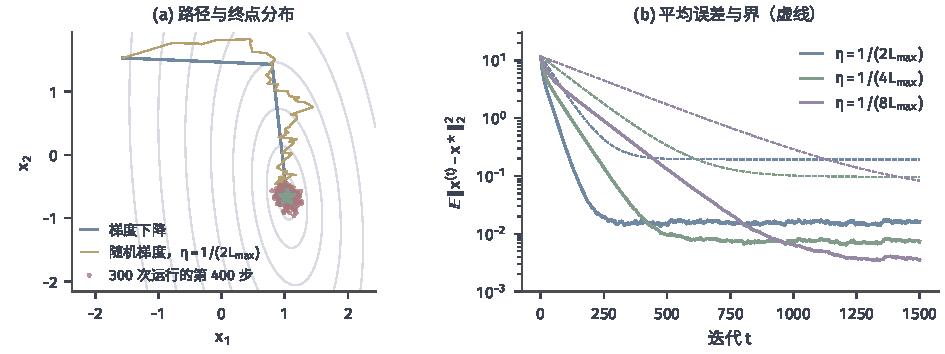
\includegraphics[width=160mm]{figures/03-optimization-evolution-and-signals/01-optimization/matplotlib/c6-sgd-noise-ball/figure.pdf}
  \caption{常数步长随机梯度下降的噪声邻域。问题是$n=40$、$d=2$的岭回归最小二乘，$\mu\approx0.304$，$L_{\max}\approx9.83$，$\sigma_\star^2\approx0.577$。(a) 灰色等高线上，蓝线为步长$1/L$的梯度下降，黄线为步长$1/(2L_{\max})$的一条随机梯度路径，红点为从最小点出发的$300$次独立运行在第$400$步的位置。(b) $400$次运行的平均平方距离（实线）与定理~\ref{thm:opt-sto-constant-step}的上界（同色虚线）。}
  \label{fig:opt-sto-noise-ball}
\end{figure*}

\paragraph{有限步结论与长期收敛}
式~\eqref{eq:opt-sto-noise-ball}是关于每个固定$t$的期望的界，不是关于单条路径的界。要让期望误差趋于零，必须让步长趋于零，下一小节给出具体的调度和速率。经典的\term{随机逼近}（stochastic approximation）理论还研究另一个问题：在$\sum_t\eta^{(t)}=\infty$、$\sum_t(\eta^{(t)})^2<\infty$等条件下，迭代点是否\emph{几乎必然}收敛\scite{math-robbins1951stochastic}。那需要鞅收敛定理来控制累积噪声，不能只靠逐步取期望得到，归第~\ref{chap:stochastic-processes-and-approximation}章。本章不把这些步长条件当作已证明的收敛保证使用。

\subsection{步长调度}
\label{sec:opt-sto-schedules}

\paragraph{几种调度规则}
定理~\ref{thm:opt-sto-constant-step}说明步长同时控制两件事：初始误差消退的速度和噪声累积的水平。按迭代推进改变步长的规则称为步长调度，在机器学习中通常叫\term{学习率调度}（learning rate scheduling）。常见的有四类。\emph{常数}步长最简单，误差停在与$\eta$成正比的平台上。\emph{预定递减}步长如$\eta^{(t)}=\eta^{(0)}/(1+t/t_0)$，事先写成迭代次数的函数。\emph{分段}步长在若干预定时刻把步长乘以一个因子，例如每$K$步减半。\emph{按观测调整}的规则读取一个监测量，例如若干步内目标估计不再下降就减小步长。

\paragraph{调度的时钟}
每种调度都依赖一个“时钟”$t$，它可以数样本读取次数、参数更新次数或数据遍历次数，三者在批量和微批量下并不相同。批量为$b$时，“每$500$步减半”与“每读取$500$个样本减半”相差$b$倍。把一个批量拆成几个微批量累积时（第~\ref{sec:opt-sto-minibatch}节），若在每个微批量之后推进时钟，步长就会比预定的更快地减小。改变时钟就改变了实际执行的算法，报告调度时必须同时说明时钟的单位。

按观测调整的规则还有一层需要检查：步长必须在抽取本步读数之前确定。若用本步读数本身决定本步步长，例如读数大时缩小步长，那么$\mathbb E_t[\eta^{(t)}\bm g^{(t)}]\neq\eta^{(t)}\nabla f(\bm x^{(t)})$，前面的单步分析就不再适用。用上一步或单独一批样本上的监测量调整则没有这个问题。

\paragraph{递减步长的速率}
在强凸情形下，适当的递减步长让期望误差以$1/t$的速度趋于零。下面的定理把这一点从同一条递推中推出。

\begin{theorem}[递减步长的期望误差]
\label{thm:opt-sto-decreasing}
在引理~\ref{lem:opt-sto-distance}的条件下设$\mu>0$，取$t_0\geq4L_{\max}/\mu$与
\[
  \eta^{(t)}=\frac{2}{\mu(t+t_0)} .
\]
则对一切$t\geq0$，$\mathbb E\lVert\bm x^{(t)}-\bm x^\star\rVert_2^2\leq\dfrac{\nu}{t+t_0}$，其中$\nu=\max\bigl\{t_0\lVert\bm x^{(0)}-\bm x^\star\rVert_2^2,\ 8\sigma_\star^2/\mu^2\bigr\}$。
\end{theorem}

\begin{proof}
由$t_0\geq4L_{\max}/\mu$，$\eta^{(t)}\leq2/(\mu t_0)\leq1/(2L_{\max})$，所以与定理~\ref{thm:opt-sto-constant-step}的证明相同，$a_t=\mathbb E\lVert\bm x^{(t)}-\bm x^\star\rVert_2^2$满足$a_{t+1}\leq(1-\mu\eta^{(t)})a_t+2(\eta^{(t)})^2\sigma_\star^2$。对$t$归纳。$t=0$时$a_0\leq\nu/t_0$由$\nu$的定义成立。设$a_t\leq\nu/k$，$k=t+t_0\geq4$，则$1-\mu\eta^{(t)}=1-2/k\geq0$，
\[
  a_{t+1}\leq\Bigl(1-\frac2k\Bigr)\frac\nu k+\frac{8\sigma_\star^2}{\mu^2k^2}
  \leq\frac{(k-2)\nu}{k^2}+\frac{\nu}{k^2}=\frac{(k-1)\nu}{k^2}\leq\frac{\nu}{k+1},
\]
其中第二步用$8\sigma_\star^2/\mu^2\leq\nu$，最后一步用$(k-1)(k+1)\leq k^2$。
\end{proof}

这条速率的代价体现在常数上：$t_0$至少是条件数$L_{\max}/\mu$的四倍，早期步长因此偏小；$\nu$中的$8\sigma_\star^2/\mu^2$说明噪声越大、曲率越小，后期误差越大。分段减半是另一种折中：在每一段用常数步长$\eta$跑到平台$2\eta\sigma_\star^2/\mu$附近，再把步长减半，平台随之减半，而下一段从更低的起点出发。图~\ref{fig:opt-sto-step-schedules}比较三种调度。常数步长最早停住；递减步长在前几百步因为步长较小而落后，此后持续下降，并始终位于定理~\ref{thm:opt-sto-decreasing}的上界之下；分段减半在每次减半后出现一个新的下降段，与递减步长在后期相当。

\begin{figure*}[!htbp]
  \centering
  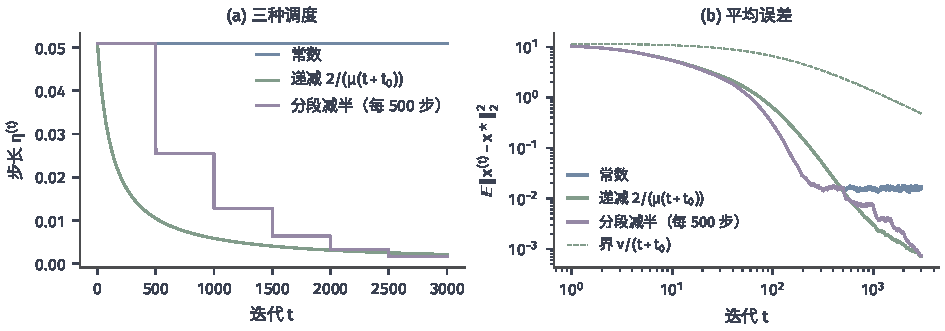
\includegraphics[width=160mm]{figures/03-optimization-evolution-and-signals/01-optimization/matplotlib/c6-step-schedules/figure.pdf}
  \caption{三种步长调度。问题同图~\ref{fig:opt-sto-noise-ball}。(a) 常数步长$\eta^{(0)}=1/(2L_{\max})\approx0.051$，递减步长$2/(\mu(t+t_0))$（$t_0=4L_{\max}/\mu\approx129$），以及每$500$步减半的分段步长。(b) $400$次运行的平均平方距离，双对数坐标；虚线是定理~\ref{thm:opt-sto-decreasing}的上界$\nu/(t+t_0)$。时钟按参数更新次数计。}
  \label{fig:opt-sto-step-schedules}
\end{figure*}

\paragraph{调度需要核验的条件}
使用任何调度，都要回到上面的递推核对三件事：每一步的步长是否满足递推成立所需的上限（这里是$\eta^{(t)}\leq1/(2L_{\max})$），步长是否在读数之前确定，以及读数是否满足所用的无偏和矩条件。步长变小时，位移变小、目标估计的波动也变小，但这只说明算法“走得慢了”，不说明已经接近最优；判断精度仍要看原目标的误差或梯度残差。另外，定理~\ref{thm:opt-sto-decreasing}给出的是期望界，一个固定的衰减公式并不自动保证每条随机路径都收敛。

\subsection{有限步误差与返回对象}
\label{sec:opt-sto-return}

前面的结论都关于“第$t$个迭代点”。实际停止时还要决定交出哪个点，而不同的返回规则配合不同的分析。本小节在凸与非凸两种情形下各给出一个有限步界，它们的返回对象并不相同。

\paragraph{凸目标与加权平均点}
不假设强凸时，到最小点的距离不再逐步收缩，但式~\eqref{eq:opt-sto-distance}中的目标差项可以被累加起来。

\begin{theorem}[凸目标的加权平均点]
\label{thm:opt-sto-convex-average}
设每个$f_i$凸且$L_{\max}$光滑，$f$有最小点$\bm x^\star$，$i^{(t)}$均匀且与历史独立，确定的步长满足$0<\eta^{(t)}\leq1/(4L_{\max})$。令$\bar{\bm x}^{(T)}=\sum_{t<T}\eta^{(t)}\bm x^{(t)}\big/\sum_{t<T}\eta^{(t)}$，则
\begin{equation}
\label{eq:opt-sto-convex-average}
  \mathbb E f(\bar{\bm x}^{(T)})-f^\star\leq\frac{\lVert\bm x^{(0)}-\bm x^\star\rVert_2^2+2\sigma_\star^2\sum_{t<T}(\eta^{(t)})^2}{\sum_{t<T}\eta^{(t)}} .
\end{equation}
\end{theorem}

\begin{proof}
在式~\eqref{eq:opt-sto-distance}中取$\mu=0$。由$\eta^{(t)}\leq1/(4L_{\max})$得$2(1-2\eta^{(t)}L_{\max})\geq1$，于是
$\eta^{(t)}\bigl(f(\bm x^{(t)})-f^\star\bigr)\leq\lVert\bm x^{(t)}-\bm x^\star\rVert_2^2-\mathbb E_t\lVert\bm x^{(t+1)}-\bm x^\star\rVert_2^2+2(\eta^{(t)})^2\sigma_\star^2$。取全期望并对$t=0,\dots,T-1$求和，距离项相消，只剩首项和一个非正的末项。最后由$f$的凸性，$f(\bar{\bm x}^{(T)})\leq\sum_t\eta^{(t)}f(\bm x^{(t)})/\sum_t\eta^{(t)}$。
\end{proof}

分子中的$\lVert\bm x^{(0)}-\bm x^\star\rVert_2^2$随总步长$\sum\eta^{(t)}$被摊薄，$2\sigma_\star^2\sum(\eta^{(t)})^2$是噪声的累积。常数步长$\eta$时右边是$\lVert\bm x^{(0)}-\bm x^\star\rVert_2^2/(\eta T)+2\eta\sigma_\star^2$，前一项要求步长大，后一项要求步长小。若预先知道总步数$T$，取$\eta=\min\{1/(4L_{\max}),\ \lVert\bm x^{(0)}-\bm x^\star\rVert_2/(\sigma_\star\sqrt{2T})\}$，代入可得
\[
  \mathbb E f(\bar{\bm x}^{(T)})-f^\star\leq\frac{4L_{\max}\lVert\bm x^{(0)}-\bm x^\star\rVert_2^2}{T}+\frac{2\sqrt2\,\sigma_\star\lVert\bm x^{(0)}-\bm x^\star\rVert_2}{\sqrt T}.
\]
无噪声时只剩$O(1/T)$，与梯度下降对凸目标的速率同阶；有噪声时$O(1/\sqrt T)$的第二项占主导。这个步长依赖于事先固定的$T$：若之后决定多跑几步，结论要按新的$T$重新核对。

\paragraph{非凸目标与随机返回点}
对非凸目标，最小点距离和目标差都不再是合适的进展度量。引理~\ref{lem:opt-sto-one-step}给出的期望下降则不依赖凸性，可以对梯度范数的平方求和。

\begin{theorem}[非凸光滑目标的随机返回点]
\label{thm:opt-sto-nonconvex}
设$f$是$L$光滑的且有下界$f_{\inf}$，读数条件无偏且$\mathbb E_t\lVert\bm g^{(t)}-\nabla f(\bm x^{(t)})\rVert_2^2\leq\sigma^2$，确定的步长满足$0<\eta^{(t)}\leq1/L$。运行结束后与算法独立地抽取$\tau\in\{0,\dots,T-1\}$，$\mathbb P(\tau=t)=\eta^{(t)}/\sum_{s<T}\eta^{(s)}$，返回$\bm x^{(\tau)}$。则
\begin{equation}
\label{eq:opt-sto-nonconvex}
  \mathbb E\lVert\nabla f(\bm x^{(\tau)})\rVert_2^2\leq\frac{2\bigl(f(\bm x^{(0)})-f_{\inf}\bigr)+L\sigma^2\sum_{t<T}(\eta^{(t)})^2}{\sum_{t<T}\eta^{(t)}} .
\end{equation}
\end{theorem}

\begin{proof}
$\eta^{(t)}\leq1/L$使式~\eqref{eq:opt-sto-one-step}中$1-L\eta^{(t)}/2\geq1/2$，于是$\tfrac{\eta^{(t)}}2\lVert\nabla f(\bm x^{(t)})\rVert_2^2\leq f(\bm x^{(t)})-\mathbb E_tf(\bm x^{(t+1)})+\tfrac L2(\eta^{(t)})^2\sigma^2$。取全期望，对$t<T$求和，目标值项相消，剩下$f(\bm x^{(0)})-\mathbb Ef(\bm x^{(T)})\leq f(\bm x^{(0)})-f_{\inf}$。由$\tau$的分布，$\mathbb E\lVert\nabla f(\bm x^{(\tau)})\rVert_2^2=\sum_t\eta^{(t)}\mathbb E\lVert\nabla f(\bm x^{(t)})\rVert_2^2/\sum_t\eta^{(t)}$，代入即得。
\end{proof}

常数步长时，右边是$2(f(\bm x^{(0)})-f_{\inf})/(\eta T)+L\eta\sigma^2$，与凸情形结构相同；取$\eta=\min\{1/L,\sqrt{2(f(\bm x^{(0)})-f_{\inf})/(L\sigma^2T)}\}$得到$O(1/T+1/\sqrt T)$的梯度平方残差\scite{ghadimi2013stochastic}。随机返回点是证明的需要：这个界控制的是梯度平方的加权平均，而不是最后一点。实践中常改为返回在独立样本上估计梯度范数最小的迭代点，那是另一个返回规则，需要另算估计误差。

\paragraph{三种返回对象}
最后一点、加权平均点和随机返回点是三个不同的随机向量，上面的定理分别只对其中一个成立。凸情形的界针对平均点；最后一点在强凸、常数步长时满足定理~\ref{thm:opt-sto-constant-step}，误差停在噪声平台上。图~\ref{fig:opt-sto-return-points}在二维最小二乘上比较它们：单次运行的最后一点剧烈波动，最后一点的平均误差停在约$8.6\times10^{-3}$；从头开始的平均点受早期远离最小点的迭代拖累，下降较慢，却没有平台；只平均后半程迭代的点兼顾两者，在$4000$步时约为$1.4\times10^{-4}$。平均能越过平台，是因为在二次目标上读数关于$\bm x$是线性的，期望迭代满足$\mathbb E\bm x^{(t+1)}-\bm x^\star=(\bm I-\eta\nabla^2f)(\mathbb E\bm x^{(t)}-\bm x^\star)$，噪声只造成围绕最小点的对称波动；这种\term{迭代平均}（iterate averaging）对二次目标与一般强凸光滑目标的渐近效果另有专门的分析\scite{polyak1992acceleration}，非二次目标上常数步长的平均点一般带有$O(\eta)$的偏差，不能把图中的结果当作普遍结论。

\begin{figure}[!htbp]
  \centering
  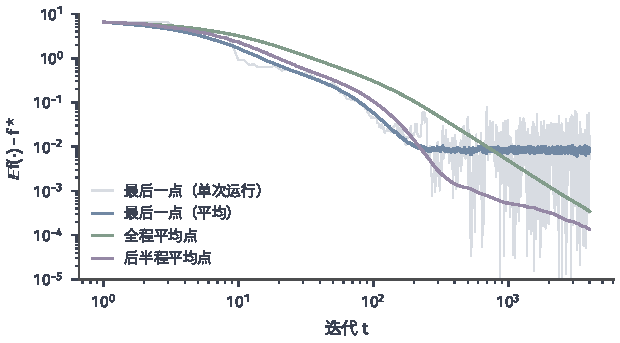
\includegraphics[width=105mm]{figures/03-optimization-evolution-and-signals/01-optimization/matplotlib/c6-return-points/figure.pdf}
  \caption{同一组运行的三种返回对象。问题同图~\ref{fig:opt-sto-noise-ball}，常数步长$1/(2L_{\max})$，$300$次运行。浅灰线为单次运行最后一点的目标差；蓝、绿、紫线分别是最后一点、全程平均点$\frac1{t+1}\sum_{s\leq t}\bm x^{(s)}$和后半程平均点$\frac{1}{t-\lfloor t/2\rfloor+1}\sum_{s=\lfloor t/2\rfloor}^{t}\bm x^{(s)}$的平均目标差，双对数坐标。}
  \label{fig:opt-sto-return-points}
\end{figure}

\paragraph{期望界的含义}
本节的结论都是期望界。若$\mathbb E[f(\bar{\bm x}^{(T)})-f^\star]\leq\varepsilon$，由Markov不等式，$\mathbb P\bigl(f(\bar{\bm x}^{(T)})-f^\star\geq\varepsilon/\delta\bigr)\leq\delta$，即以至少$1-\delta$的概率误差不超过$\varepsilon/\delta$；更紧的高概率界需要读数尾部的额外假设。期望趋于零也只蕴含依概率收敛，不蕴含几乎必然收敛，各种收敛方式之间的关系见\BookChapterRef{chap:random-variable-convergence}{卷二“随机变量的收敛与积分极限”章}。完整的鞅收敛论证、随机逼近的常微分方程解释以及长期极限都在第~\ref{chap:stochastic-processes-and-approximation}章接续，它们不是本章算法定义的前置知识。

\section{抽样与方差控制}
\label{sec:opt-sto-variance}

上一节的误差界里，噪声通过$\sigma_\star^2$或$\sigma^2$进入，并在常数步长下形成平台。本节保持目标不变，只改变读数的取得方式，看能否用额外的读取或存储换来更小的方向噪声。四种做法依次是：按不同概率抽取各项、一次读取多项、在快照点用完整梯度纠偏，以及为每一项保存一份旧梯度。前两种只把噪声按比例缩小，后两种在有限和上能让噪声随迭代趋于零。

\subsection{非均匀抽样与重加权}
\label{sec:opt-sto-importance}

\paragraph{反比权重}
各项的“分量”常常不同：最小二乘中，范数大的行梯度也大。很自然的想法是更常抽重要的项。设目标为$f(\bm x)=\frac1n\sum_i\ell_i(\bm x)+r(\bm x)$，$r$是确定的正则项，以概率$p_i>0$（$\sum_ip_i=1$）抽取下标$I$。要让读数仍条件无偏，抽到的项必须按抽样概率的倒数加权：
\begin{equation}
\label{eq:opt-sto-importance}
  \bm g=\frac{\nabla\ell_I(\bm x)}{np_I}+\nabla r(\bm x),\qquad
  \mathbb E_t[\bm g]=\sum_{i=1}^np_i\frac{\nabla\ell_i(\bm x)}{np_i}+\nabla r(\bm x)=\nabla f(\bm x).
\end{equation}
被抽得多的项每次贡献得少，被抽得少的项每次贡献得多，平均下来各项权重仍是$1/n$。这种做法是\term{重要性采样}（importance sampling）在优化中的用法。正则梯度$\nabla r(\bm x)$是确定量，不随抽样变化，每次读数只加一次，不参与重加权。

\paragraph{两项例：偏差与二阶矩}
取$n=2$，在某点$\nabla\ell_1=2$、$\nabla\ell_2=-1$，$r=0$，真梯度为$1/2$。按$p=(3/4,1/4)$抽样但不重加权，读数的平均是$\tfrac34\cdot2+\tfrac14\cdot(-1)=5/4$，偏差$3/4$。重加权后两种读数变为$2/(2\cdot\tfrac34)=4/3$与$-1/(2\cdot\tfrac14)=-2$，平均回到$1/2$。

无偏之后再看二阶矩。由式~\eqref{eq:opt-sto-importance}，
\begin{equation}
\label{eq:opt-sto-importance-moment}
  \mathbb E_t\Bigl\lVert\frac{\nabla\ell_I(\bm x)}{np_I}\Bigr\rVert_2^2=\frac1{n^2}\sum_{i=1}^n\frac{\lVert\nabla\ell_i(\bm x)\rVert_2^2}{p_i}
  \geq\Bigl(\frac1n\sum_{i=1}^n\lVert\nabla\ell_i(\bm x)\rVert_2\Bigr)^2 ,
\end{equation}
不等式由Cauchy--Schwarz不等式$\bigl(\sum_i\lVert\nabla\ell_i\rVert_2\bigr)^2=\bigl(\sum_i\sqrt{p_i}\cdot\lVert\nabla\ell_i\rVert_2/\sqrt{p_i}\bigr)^2\leq\sum_ip_i\cdot\sum_i\lVert\nabla\ell_i\rVert_2^2/p_i$得到，等号在$p_i\propto\lVert\nabla\ell_i(\bm x)\rVert_2$时成立。两项例中，均匀抽样的二阶矩为$(4+1)/2=5/2$，$p=(3/4,1/4)$时为$\tfrac34\cdot\tfrac{16}9+\tfrac14\cdot4=7/3$，最优的$p=(2/3,1/3)$给出$9/4$；而反过来取$p=(1/4,3/4)$，读数变为$4$与$-2/3$，二阶矩升到$13/3$。抽样概率很小的项一旦被抽中，读数会被放大$1/(np_i)$倍，选错概率比均匀抽样更糟。

\paragraph{按光滑常数抽样}
最优概率依赖于当前点的梯度，每步重算要读全部项，失去了抽样的意义。实用的替代是按光滑常数抽样：若$\ell_i$凸且$L_i$光滑，$r$凸且$\lambda$光滑，令$\phi_i=\ell_i/(np_i)+r$，则$f=\sum_ip_i\phi_i$，读数恰为$\nabla\phi_I(\bm x)$，$\phi_i$凸且$\bigl(L_i/(np_i)+\lambda\bigr)$光滑。在引理~\ref{lem:opt-sto-distance}的证明中把均匀平均换成$p$加权平均，结论不变，只需把$L_{\max}$换成$\max_iL_i/(np_i)+\lambda$、把$\sigma_\star^2$换成$\sigma_{\star,p}^2=\sum_ip_i\lVert\nabla\phi_i(\bm x^\star)\rVert_2^2$。取$p_i=L_i/\sum_jL_j$时，前者变为平均光滑常数$\bar L+\lambda$，$\bar L=\frac1n\sum_iL_i$。少数几项特别陡时，$\bar L$远小于$\max_iL_i$，允许的步长和定理~\ref{thm:opt-sto-decreasing}中的$t_0$都随之改善\scite{needell2016stochastic}。代价是$\sigma_{\star,p}^2$可能变大：最小点处梯度大的项未必是光滑常数大的项。

图~\ref{fig:opt-sto-importance}展示这一取舍。数据中前$4$行被放大$6$倍，$L_{\max}\approx80.6$，而平均光滑常数只有约$5.64$。按$p_i\propto\lVert\bm a_i\rVert_2^2$抽样并重加权后，$t_0$从约$458$降到约$32$，误差早早开始下降；但最小点处的噪声从$\sigma_\star^2\approx0.645$升到$\sigma_{\star,p}^2\approx1.12$，到$3000$步时均匀抽样反而略低。不重加权的运行则收敛到另一个点，误差停在红色虚线处，那是把加权平均$\sum_ip_i\nabla\ell_i$当作梯度时的驻点。

\begin{figure*}[!htbp]
  \centering
  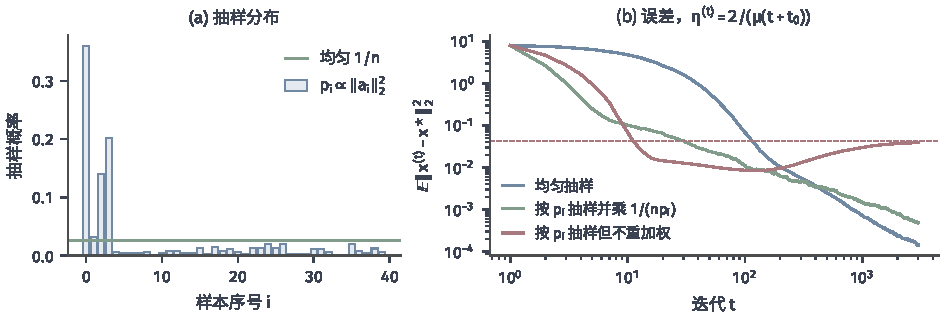
\includegraphics[width=160mm]{figures/03-optimization-evolution-and-signals/01-optimization/matplotlib/c6-importance-sampling/figure.pdf}
  \caption{非均匀抽样。$n=40$、$d=2$的岭回归最小二乘，前$4$行放大$6$倍。(a) 按$p_i\propto\lVert\bm a_i\rVert_2^2$的抽样概率与均匀概率$1/n$。(b) $300$次运行的平均平方距离，双对数坐标，三条曲线都用递减步长$2/(\mu(t+t_0))$：蓝线为均匀抽样，$t_0=4L_{\max}/\mu\approx458$；绿线按$p_i$抽样并乘$1/(np_i)$，$t_0=4(\bar L+\lambda)/\mu\approx32$；红线按$p_i$抽样但不重加权，步长同蓝线，它收敛到有偏的驻点，红色虚线标出该点到$\bm x^\star$的平方距离。}
  \label{fig:opt-sto-importance}
\end{figure*}

\paragraph{抽样本身的成本}
非均匀抽样还要算上维护分布的成本。概率固定时，用别名表可以$O(n)$预处理、$O(1)$抽样；概率随迭代变化时，常用树结构在$O(\log n)$时间内更新与抽样。若概率要靠估计各项的当前梯度来设定，估计所需的读取也要计入。比较抽样策略时，应在同样的读取与计算预算下比较误差，而不是只比较迭代次数。

\subsection{小批量与梯度累积}
\label{sec:opt-sto-minibatch}

\paragraph{独立平均的方差}
最直接的降噪办法是一次读多项再平均。设给定历史后，$i_1,\dots,i_b$相互独立且都在$\{1,\dots,n\}$上均匀分布（有放回抽样），\term{小批量}（mini-batch）读数为$\bm g_B=\frac1b\sum_{k=1}^b\nabla f_{i_k}(\bm x)$。记$\bm\xi_k=\nabla f_{i_k}(\bm x)-\nabla f(\bm x)$，则
\[
  \mathbb E_t\lVert\bm g_B-\nabla f(\bm x)\rVert_2^2=\frac1{b^2}\sum_{k=1}^b\mathbb E_t\lVert\bm\xi_k\rVert_2^2+\frac1{b^2}\sum_{k\neq l}\mathbb E_t\langle\bm\xi_k,\bm\xi_l\rangle=\frac{\sigma^2(\bm x)}{b},
\]
其中$\sigma^2(\bm x)=\frac1n\sum_i\lVert\nabla f_i(\bm x)-\nabla f(\bm x)\rVert_2^2$是单项读数的方差。交叉项消失靠的是条件独立：$\mathbb E_t\langle\bm\xi_k,\bm\xi_l\rangle=\langle\mathbb E_t\bm\xi_k,\mathbb E_t\bm\xi_l\rangle=0$。所以前面所有误差界中的$\sigma^2$都可以换成$\sigma^2/b$，噪声平台按$1/b$缩小。

独立性不满足时公式要改。无放回地抽取$b$个不同下标，交叉项变为负值，方差为$\frac{\sigma^2(\bm x)}b\cdot\frac{n-b}{n-1}$，$b=n$时恰好为零。三点例中$b=2$：有放回时方差为$\tfrac{14}3\cdot\tfrac12=\tfrac73$；无放回时三种组合$\{1,2\},\{1,3\},\{2,3\}$的平均$c$分别为$0.5,2.5,3$，与$2$的差的平方平均为$(2.25+0.25+1)/3=7/6$，与公式$\tfrac73\cdot\tfrac12$一致。反过来，若批内样本高度相关，例如把同一个样本重复$b$次，平均就毫无降噪作用，方差仍是$\sigma^2$。图~\ref{fig:opt-sto-minibatch}在$n=200$的最小二乘上核对了两条公式。

\begin{figure}[!htbp]
  \centering
  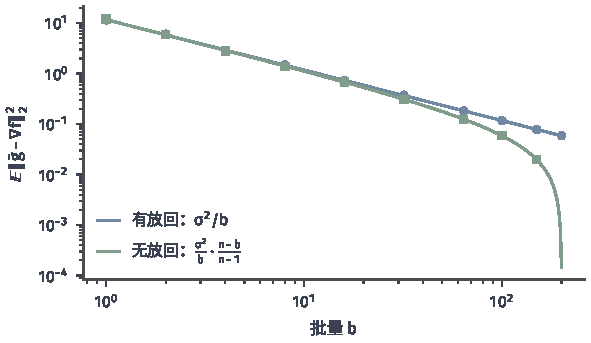
\includegraphics[width=100mm]{figures/03-optimization-evolution-and-signals/01-optimization/matplotlib/c6-minibatch-variance/figure.pdf}
  \caption{小批量读数的方差随批量$b$的变化。最小二乘$n=200$、$d=5$，在$\bm x=\bm0$处单项方差$\sigma^2\approx11.7$。实线为公式，圆点（有放回）与方块（无放回）为每个$b$各$4000$次抽样的经验值，双对数坐标。有放回时方差严格按$1/b$下降；无放回时在$b$接近$n$处迅速降到零，$b=n$时为零未画出。}
  \label{fig:opt-sto-minibatch}
\end{figure}

\paragraph{批量不能消除偏差}
批量平均只压低式~\eqref{eq:opt-sto-reading-split}中的噪声$\bm\xi$，对条件偏差$\bm\beta$毫无作用：$b$个有相同偏差的读数，平均后偏差不变。另外，批量为$b$的一步要读取$b$项，期望下降量却至多是精确梯度步的下降量。噪声已不是主要限制时，继续增大批量只是用$b$倍的读取换取几乎相同的一步，第~\ref{sec:opt-sto-cost}节会把这一点画成读取量随批量变化的曲线。

\paragraph{梯度累积}
批量受内存限制时，可以把它拆成若干微批量依次计算再合并，这称为\term{梯度累积}（gradient accumulation）。设一个批量$B$拆为$K$个不相交的微批量$B_1,\dots,B_K$，大小$n_j=|B_j|$，$N=\sum_jn_j$。要与一次读完$B$等价，必须满足下面算法中的约定。

\begin{algorithm}[梯度累积的一次更新]
\label{alg:opt-sto-accumulation}
\begin{algorithmic}[1]
\Require 当前参数$\bm x$（整个窗口内冻结），微批量$B_1,\dots,B_K$，步长$\eta$，确定的正则项$r$
\Ensure 新参数，以及只推进一次的调度时钟与优化器状态
\State $\bm s\gets\bm0$
\For{$j=1,\dots,K$}
  \State 在同一个$\bm x$处计算微批量平均$\bar{\bm g}_j=\frac1{n_j}\sum_{i\in B_j}\nabla\ell_i(\bm x)$
  \State $\bm s\gets\bm s+n_j\bar{\bm g}_j$ \Comment{按样本数加权}
\EndFor
\State $\bm g\gets\bm s/N+\nabla r(\bm x)$ \Comment{正则梯度只加一次}
\State $\bm x\gets\bm x-\eta\bm g$；调度时钟、动量与二阶统计各推进一次
\end{algorithmic}
\end{algorithm}

按样本数加权是必要的。若$n_1=2$、$n_2=1$，两组平均分别为$1$和$4$，正确的批量平均是$(2\cdot1+1\cdot4)/3=2$，直接平均两组得到$5/2$，相当于给第二组的样本加了双倍权重。等价性还要求窗口内每个样本被求值的函数和求值点与一次读完时相同：如果网络中有依赖批统计量的批归一化，或者随机失活在各微批量用了不同的随机状态，微批量上的函数就与大批量上的不同，结果不再一致。梯度累积减少的是同时驻留的中间结果，即存储；它仍要读取$N$项、做$K$次前向与反向计算，总读取量并不减少。

\subsection{SVRG}
\label{sec:opt-sto-svrg}

\paragraph{控制变量}
批量降噪需要每步多读，而且噪声只按比例缩小。另一种思路来自蒙特卡罗估计中的\term{控制变量}（control variate）：要估计$\mathbb E[Z]$，若有一个与$Z$高度相关、且期望$\mathbb E[Y]$已知的量$Y$，那么$Z-Y+\mathbb E[Y]$的期望仍是$\mathbb E[Z]$，方差却是$\mathbb E\lVert(Z-\mathbb EZ)-(Y-\mathbb EY)\rVert_2^2$，$Z$与$Y$越接近就越小。在有限和上，取$Z=\nabla f_i(\bm x)$，$Y=\nabla f_i(\tilde{\bm x})$为同一项在一个参考点$\tilde{\bm x}$处的梯度，它的期望$\nabla f(\tilde{\bm x})$只要在参考点算一次完整梯度就知道了。这就是\term{方差缩减}（variance reduction）方法SVRG的读数\scite{johnson2013accelerating}：
\begin{equation}
\label{eq:opt-sto-svrg}
  \bm v=\nabla f_i(\bm x)-\nabla f_i(\tilde{\bm x})+\tilde{\bm\mu},\qquad\tilde{\bm\mu}=\nabla f(\tilde{\bm x}).
\end{equation}
$i$均匀且与历史独立时，$\mathbb E_t[\bm v]=\nabla f(\bm x)-\nabla f(\tilde{\bm x})+\tilde{\bm\mu}=\nabla f(\bm x)$，读数条件无偏。

\begin{algorithm}[SVRG]
\label{alg:opt-sto-svrg}
\begin{algorithmic}[1]
\Require 初始快照$\tilde{\bm x}^{(0)}$，步长$\eta$，内循环长度$m$，外循环轮数$S$
\Ensure 最后的快照$\tilde{\bm x}^{(S)}$
\For{$s=0,1,\dots,S-1$}
  \State 计算完整梯度$\tilde{\bm\mu}=\nabla f(\tilde{\bm x}^{(s)})$ \Comment{读取$n$项}
  \State $\bm x^{(0)}\gets\tilde{\bm x}^{(s)}$
  \For{$k=0,1,\dots,m-1$}
    \State 均匀抽取$i$，$\bm v\gets\nabla f_i(\bm x^{(k)})-\nabla f_i(\tilde{\bm x}^{(s)})+\tilde{\bm\mu}$
    \State $\bm x^{(k+1)}\gets\bm x^{(k)}-\eta\bm v$
  \EndFor
  \State 均匀抽取$k\in\{0,\dots,m-1\}$，令$\tilde{\bm x}^{(s+1)}\gets\bm x^{(k)}$ \Comment{实践中常取$\bm x^{(m)}$}
\EndFor
\end{algorithmic}
\end{algorithm}

算法的状态是快照$\tilde{\bm x}$、快照处的完整梯度$\tilde{\bm\mu}$和当前点$\bm x$，存储$O(d)$。每步内循环要计算两个单项梯度；若改为保存全部$\nabla f_i(\tilde{\bm x})$，可省去一次计算，但存储变为$O(nd)$（对线性模型只需保存$n$个标量残差）。一个外循环的读取量是$n+2m$。

\paragraph{方差为何趋于零}
读数的噪声是$\bm v-\nabla f(\bm x)=[\nabla f_i(\bm x)-\nabla f_i(\tilde{\bm x})]-\mathbb E_t[\nabla f_i(\bm x)-\nabla f_i(\tilde{\bm x})]$。随机向量减去自身均值后，二阶矩不超过原二阶矩，所以若每项$L_{\max}$光滑，
\[
  \mathbb E_t\lVert\bm v-\nabla f(\bm x)\rVert_2^2\leq\frac1n\sum_{i=1}^n\lVert\nabla f_i(\bm x)-\nabla f_i(\tilde{\bm x})\rVert_2^2\leq L_{\max}^2\lVert\bm x-\tilde{\bm x}\rVert_2^2 .
\]
当前点与快照都接近最小点时，读数噪声随之趋于零，这是普通随机梯度做不到的：后者在最小点处的方差仍是$\sigma_\star^2$。三点例把这一点推到极端：$\nabla f_i(x)-\nabla f_i(\tilde x)=x-\tilde x$与$i$无关，于是$v=x-\tilde x+(\tilde x-2)=x-2$，每一步读数都精确等于真梯度。一般问题中各项曲率不同，噪声不为零，但会随$\bm x,\tilde{\bm x}\to\bm x^\star$而缩小。

\paragraph{强凸情形的线性收敛}
用引理~\ref{lem:opt-sto-cocoercive}可以把读数的二阶矩与目标差联系起来，再沿用距离递推。

\begin{lemma}[SVRG读数的二阶矩]
\label{lem:opt-sto-svrg-moment}
设每个$f_i$凸且$L_{\max}$光滑，$\bm x^\star$是$f$的最小点。则式~\eqref{eq:opt-sto-svrg}满足
\[
  \mathbb E_t\lVert\bm v\rVert_2^2\leq4L_{\max}\bigl(f(\bm x)-f^\star\bigr)+4L_{\max}\bigl(f(\tilde{\bm x})-f^\star\bigr).
\]
\end{lemma}

\begin{proof}
把$\bm v$写成$[\nabla f_i(\bm x)-\nabla f_i(\bm x^\star)]-[\nabla f_i(\tilde{\bm x})-\nabla f_i(\bm x^\star)-\nabla f(\tilde{\bm x})]$，用$\lVert\bm u-\bm w\rVert_2^2\leq2\lVert\bm u\rVert_2^2+2\lVert\bm w\rVert_2^2$。第一部分由引理~\ref{lem:opt-sto-cocoercive}及$\nabla f(\bm x^\star)=\bm0$，平均后不超过$2L_{\max}(f(\bm x)-f^\star)$。第二部分是随机向量$\nabla f_i(\tilde{\bm x})-\nabla f_i(\bm x^\star)$减去它的均值$\nabla f(\tilde{\bm x})$，二阶矩不超过未中心化的二阶矩，同理不超过$2L_{\max}(f(\tilde{\bm x})-f^\star)$。
\end{proof}

\begin{theorem}[SVRG的线性收敛]
\label{thm:opt-sto-svrg}
设每个$f_i$凸且$L_{\max}$光滑，$f$是$\mu$强凸的，$0<\eta<1/(4L_{\max})$，$m$满足
\[
  \alpha=\frac{1}{\mu\eta(1-2L_{\max}\eta)m}+\frac{2L_{\max}\eta}{1-2L_{\max}\eta}<1 .
\]
则算法~\ref{alg:opt-sto-svrg}满足$\mathbb Ef(\tilde{\bm x}^{(s+1)})-f^\star\leq\alpha\bigl(\mathbb Ef(\tilde{\bm x}^{(s)})-f^\star\bigr)$。
\end{theorem}

\begin{proof}
固定一个外循环，记$\tilde{\bm x}=\tilde{\bm x}^{(s)}$。与引理~\ref{lem:opt-sto-distance}的证明相同地展开$\lVert\bm x^{(k+1)}-\bm x^\star\rVert_2^2$，内积项用凸性$\langle\nabla f(\bm x),\bm x-\bm x^\star\rangle\geq f(\bm x)-f^\star$，平方项用引理~\ref{lem:opt-sto-svrg-moment}，得到
\[
  \begin{aligned}
    \mathbb E_k\lVert\bm x^{(k+1)}-\bm x^\star\rVert_2^2
    &\leq\lVert\bm x^{(k)}-\bm x^\star\rVert_2^2-2\eta(1-2L_{\max}\eta)\bigl(f(\bm x^{(k)})-f^\star\bigr)\\
    &\quad+4L_{\max}\eta^2\bigl(f(\tilde{\bm x})-f^\star\bigr).
  \end{aligned}
\]
对$k=0,\dots,m-1$取期望求和，距离项相消，再用$\bm x^{(0)}=\tilde{\bm x}$与强凸性$\lVert\tilde{\bm x}-\bm x^\star\rVert_2^2\leq\tfrac2\mu(f(\tilde{\bm x})-f^\star)$：
\[
  2\eta(1-2L_{\max}\eta)\sum_{k=0}^{m-1}\mathbb E\bigl(f(\bm x^{(k)})-f^\star\bigr)\leq\Bigl(\frac2\mu+4L_{\max}\eta^2m\Bigr)\bigl(f(\tilde{\bm x})-f^\star\bigr).
\]
新快照在$\bm x^{(0)},\dots,\bm x^{(m-1)}$中均匀选取，左边求和恰为$m\,\mathbb E(f(\tilde{\bm x}^{(s+1)})-f^\star)$的$2\eta(1-2L_{\max}\eta)$倍。两边相除即得$\alpha$。
\end{proof}

以$\kappa_{\max}=L_{\max}/\mu$计，取$\eta=1/(10L_{\max})$，$1-2L_{\max}\eta=0.8$，第二项为$0.25$；取$m=50\kappa_{\max}$，第一项为$1/(\tfrac1{10\kappa_{\max}}\cdot0.8\cdot50\kappa_{\max})=0.25$，于是$\alpha=1/2$。每个外循环把目标差减半，读取量为$n+2m=n+100\kappa_{\max}$，达到精度$\varepsilon$总共需要$O\bigl((n+\kappa_{\max})\log(1/\varepsilon)\bigr)$次读取。作为对照，梯度下降需要$O(n\kappa\log(1/\varepsilon))$次读取，普通随机梯度由定理~\ref{thm:opt-sto-decreasing}需要$O(\sigma_\star^2/(\mu^2\varepsilon))$量级的迭代：前者每步太贵，后者对$\varepsilon$不是对数依赖。定理的常数偏保守，实践中常用更大的步长，取最后一点作为新快照，并把$m$取为$n$的若干倍；这些改动需要另行核验。

\subsection{SAGA}
\label{sec:opt-sto-saga}

\paragraph{用梯度记忆代替快照}
SVRG的参考点每隔$m$步才更新一次，而且每次更新要读全部数据。SAGA改为给每一项各存一份“最近一次读到的梯度”$\bm\phi_i$，并维护它们的平均$\bar{\bm\phi}=\frac1n\sum_i\bm\phi_i$\scite{defazio2014saga}。抽到第$j$项时，用新旧读数之差纠偏：
\begin{equation}
\label{eq:opt-sto-saga}
  \bm v=\nabla f_j(\bm x)-\bm\phi_j+\bar{\bm\phi},
\end{equation}
然后用$\bm v$更新参数，再把$\bm\phi_j$替换为$\nabla f_j(\bm x)$、把$\bar{\bm\phi}$加上$(\nabla f_j(\bm x)-\bm\phi_j)/n$。

\begin{algorithm}[SAGA]
\label{alg:opt-sto-saga}
\begin{algorithmic}[1]
\Require 初值$\bm x^{(0)}$，步长$\eta$，轮数$T$
\Ensure 最后一点$\bm x^{(T)}$
\State 对每个$i$置$\bm\phi_i\gets\nabla f_i(\bm x^{(0)})$，$\bar{\bm\phi}\gets\frac1n\sum_i\bm\phi_i$ \Comment{读取$n$项}
\For{$t=0,1,\dots,T-1$}
  \State 均匀抽取$j$，计算$\bm u\gets\nabla f_j(\bm x^{(t)})$
  \State $\bm v\gets\bm u-\bm\phi_j+\bar{\bm\phi}$ \Comment{用更新前的平均}
  \State $\bm x^{(t+1)}\gets\bm x^{(t)}-\eta\bm v$
  \State $\bar{\bm\phi}\gets\bar{\bm\phi}+(\bm u-\bm\phi_j)/n$，$\bm\phi_j\gets\bm u$
\EndFor
\end{algorithmic}
\end{algorithm}

\paragraph{哪一个平均保证无偏}
算法中构造$\bm v$用的是\emph{更新前}的$\bar{\bm\phi}$。此时表$\bm\phi_1,\dots,\bm\phi_n$由历史决定，$\mathbb E_t[\nabla f_j(\bm x)-\bm\phi_j]=\nabla f(\bm x)-\bar{\bm\phi}$，加上$\bar{\bm\phi}$后正好是$\nabla f(\bm x)$。若先更新平均再构造方向，读数变为$\bm v'=\bm v+(\nabla f_j(\bm x)-\bm\phi_j)/n$，条件期望多出$(\nabla f(\bm x)-\bar{\bm\phi})/n$，只要表还没有追上当前梯度就有偏。条件无偏来自“新读数减去同一项的旧读数”，旧读数的平均必须是构造方向那一刻的已知量。

三点例同样能看清记忆的作用。设第$i$项上次被读取时参数为$x_{k_i}$，则$\phi_i=x_{k_i}-c_i$，代入式~\eqref{eq:opt-sto-saga}得$v=x-x_{k_j}+\frac13\sum_ix_{k_i}-2$。数据值$c_i$完全消去，噪声只来自各项记录的“年龄”不同。表刚初始化时所有$x_{k_i}$相同，$v$恰为真梯度；随着迭代收敛，各次记录的参数彼此接近，噪声也趋于零。

\paragraph{误差的两个来源与代价}
分析SAGA时，误差不只在参数上，还在表里：表中的旧梯度离$\nabla f_i(\bm x^\star)$越远，读数噪声越大。因此收敛证明使用同时包含两部分的势函数，形如$\lVert\bm x-\bm x^\star\rVert_2^2+c\cdot\frac1n\sum_i\lVert\bm\phi_i-\nabla f_i(\bm x^\star)\rVert_2^2$。在每项凸且$L_{\max}$光滑、$f$为$\mu$强凸的条件下，取步长$1/(3L_{\max})$时，期望距离按每步$1-\min\{1/(4n),\mu/(3L_{\max})\}$的比率线性收敛\scite{defazio2014saga}。$n$大时比率由$1/(4n)$决定，即大约每遍历一次数据误差缩小一个常数因子，与SVRG的总读取量同阶。

图~\ref{fig:opt-sto-variance-reduction}在$n=200$、$d=10$的岭逻辑回归上比较五种方法，横轴统一为读取量。常数步长的随机梯度很快停在约$10^{-2}$的平台，递减步长继续缓慢下降；梯度下降每步读$n$项，在$30$遍数据内只走$30$步。SVRG与SAGA则保持线性收敛，(b)显示其原因：普通随机梯度的方向方差始终约为$1$，SVRG的方差在每次快照时归零、随后回升，整体逐轮下降，SAGA的方差随表的更新稳步下降。

\begin{figure*}[!htbp]
  \centering
  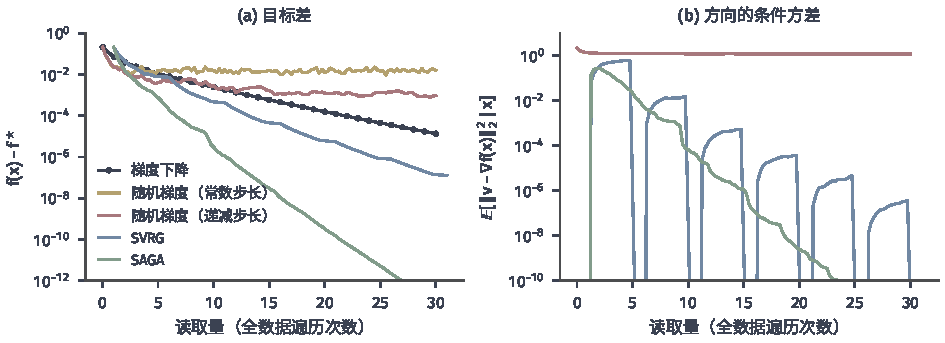
\includegraphics[width=160mm]{figures/03-optimization-evolution-and-signals/01-optimization/matplotlib/c6-variance-reduction/figure.pdf}
  \caption{方差缩减方法与随机梯度的比较。岭逻辑回归，$n=200$，$d=10$，$\lambda=0.05$，$L\approx0.71$，$L_{\max}\approx10.0$，$8$个随机种子平均。横轴为读取量除以$n$；梯度下降每步读$n$项，SVRG每个外循环读$n+2m$项（$m=2n$），SAGA初始化读$n$项、此后每步读$1$项。步长：梯度下降$1/L$，随机梯度$1/(2L_{\max})$（递减版本再除以$1+t/(2n)$），SVRG与SAGA均为实验取值$1/(3L_{\max})$，比定理~\ref{thm:opt-sto-svrg}所需的保守常数大。(a) 目标差；(b) 当前点处方向读数的条件方差，由全部$n$项精确计算。}
  \label{fig:opt-sto-variance-reduction}
\end{figure*}

代价方面，SAGA每步只读一项、不需要周期性的全数据遍历，但要存储$n$个梯度，一般为$O(nd)$；对线性模型$\nabla f_i(\bm x)=\ell_i'(\bm a_i^\top\bm x)\bm a_i+\lambda\bm x$，只需存$n$个标量$\ell_i'$。更根本的限制是适用范围：SVRG和SAGA都要求能反复访问同一项，这是有限和的结构。对只能不断获得新样本的期望目标~\eqref{eq:opt-sto-expectation}，每个样本只见一次，既没有可复用的旧读数，也无法计算快照处的完整梯度，两种方法不能原样使用。

\section{历史信息与自适应更新}
\label{sec:opt-sto-adaptive}

上一节用历史读数纠正方向的偏离。本节研究历史读数的另一种用法：根据过去读数的幅度为各个坐标或各个矩阵方向确定尺度。这些机制同样可以用于精确梯度，第~\ref{chap:opt-smooth}章的动量就是用历史形成方向的例子；与随机读数结合时，尺度本身也成了随机量，原来的偏差与收敛分析需要重新检查。本节只收纳确实维护历史统计的方法。步长调度已在第~\ref{sec:opt-sto-schedules}节随随机梯度建立，裁剪和替代梯度改变的是读数本身，放在第~\ref{sec:opt-sto-direction}节。

\subsection{累计尺度与AdaGrad}
\label{sec:opt-sto-adagrad}

\paragraph{逐坐标的累计尺度}
设想一个文本分类问题，特征是词是否出现。常见词几乎在每个样本中出现，对应坐标的读数每步都不为零；罕见词偶尔出现，对应坐标大多数时候读数为零。用同一个步长，常见词坐标被频繁推动，罕见词坐标几乎不动。AdaGrad为每个坐标记录读数平方的累计和，用它的平方根去除当前读数\scite{duchi2011adagrad}。取$\bm v^{(0)}=\bm0$、步长$\eta>0$与稳定常数$\epsilon>0$，每轮依次执行
\begin{equation}
\label{eq:opt-sto-adagrad}
  \bm v^{(t+1)}=\bm v^{(t)}+\bm g^{(t)}\odot\bm g^{(t)},\qquad
  \bm x^{(t+1)}=\bm x^{(t)}-\eta\,\frac{\bm g^{(t)}}{\sqrt{\bm v^{(t+1)}}+\epsilon},
\end{equation}
其中$\odot$、平方根和除法都逐坐标进行。顺序是先读数、再用本轮读数更新统计、最后用新统计缩放本轮读数。稳定常数放在根号外，只为避免分母为零；有的实现把它放在根号内，两者在$\bm v$很小时行为不同，须按实际实现记录。

这里的尺度来自读数的历史二阶矩，一般不是目标的Hessian。对一维二次函数$f(x)=\tfrac h2x^2$，精确梯度为$hx$，累计量是$\sum_sh^2(x^{(s)})^2$，它同时取决于曲率$h$和走过的路径，并不等于$h$。逐坐标除以历史幅度，可以看作一种随时间变化的对角缩放，但它不是对固定曲率的近似。

\paragraph{两个坐标的短序列}
取$\eta=1$、忽略$\epsilon$。坐标$1$每轮读数都是$1$，坐标$2$只在$t=0$与$t=4$读数为$1$，其余时刻为零。表~\ref{tab:opt-sto-adagrad-steps}列出各轮实际作用在非零读数上的系数$\eta/\sqrt{v_k^{(t+1)}}$。坐标$1$的系数按$1/\sqrt{t+1}$持续缩小，到第$4$轮是$0.447$；坐标$2$的累计量只在它真正出现时增长，第$4$轮的系数仍有$0.707$。稀疏坐标因此保留了较大的有效步长。表中右侧是下一小节的RMSProp（$\rho=0.9$），供比较。

\begin{table}[!htbp]
  \centering
  \small
  \caption{两个坐标上AdaGrad与RMSProp的有效系数$\eta/\sqrt{v_k^{(t+1)}}$（$\eta=1$，忽略稳定项）。坐标$1$每轮读数为$1$；坐标$2$只在$t=0,4$读数为$1$，其余轮读数为零、不发生位移，记为“—”。}
  \label{tab:opt-sto-adagrad-steps}
  \begin{tabular}{ccccc}
    \toprule
    & \multicolumn{2}{c}{AdaGrad} & \multicolumn{2}{c}{RMSProp}\\
    \cmidrule(lr){2-3}\cmidrule(lr){4-5}
    轮次$t$ & 坐标$1$ & 坐标$2$ & 坐标$1$ & 坐标$2$\\
    \midrule
    $0$ & $1.000$ & $1.000$ & $3.162$ & $3.162$\\
    $1$ & $0.707$ & — & $2.294$ & —\\
    $2$ & $0.577$ & — & $1.921$ & —\\
    $3$ & $0.500$ & — & $1.705$ & —\\
    $4$ & $0.447$ & $0.707$ & $1.563$ & $2.457$\\
    $5$ & $0.408$ & — & $1.461$ & —\\
    \bottomrule
  \end{tabular}
\end{table}

\paragraph{存储与长期缩步}
AdaGrad的额外状态是一个$d$维向量，每轮额外计算$O(d)$。累计量只增不减，因此每个坐标的有效步长单调变小。对读数幅度大致恒定的坐标，有效步长按$1/\sqrt t$衰减，这与凸在线问题的需要相符；但对非凸训练，早期的大读数会永久压低后期步长，算法可能在远未收敛时就几乎停止移动。

\paragraph{保证的范围}
AdaGrad最初的分析针对凸的在线学习：在可行域有界、读数有界等条件下，累计损失与最优固定决策之差按$O(\sqrt T)$增长，且对稀疏读数有更好的常数\scite{duchi2011adagrad}。确定性光滑问题、随机凸问题和非凸问题上的分析各有不同的假设与结论，引用时须注明属于哪一种。仅从更新形式不能推出“对任何问题都比梯度下降快”：逐坐标缩放只有在问题的难点与坐标轴对齐时才有明显收益，图~\ref{fig:opt-sto-adaptive-paths}会给出反例。

\subsection{衰减统计与Adam}
\label{sec:opt-sto-adam}

\paragraph{RMSProp：让旧尺度逐渐遗忘}
AdaGrad的累计量无法忘记早期的大读数。RMSProp把累计和换成\term{指数移动平均}（exponential moving average）\scite{hinton2012rmsprop}：
\[
\begin{aligned}
  \bm v^{(t+1)}&=\rho\bm v^{(t)}+(1-\rho)\bm g^{(t)}\odot\bm g^{(t)},\qquad\rho\in[0,1),\\
  \bm x^{(t+1)}&=\bm x^{(t)}-\eta^{(t)}\frac{\bm g^{(t)}}{\sqrt{\bm v^{(t+1)}}+\epsilon}.
\end{aligned}
\]
展开递推，$\bm v^{(t+1)}=(1-\rho)\sum_{s\leq t}\rho^{t-s}\bm g^{(s)}\odot\bm g^{(s)}$，大约只记住最近$1/(1-\rho)$轮。读数恒为$g$时$\bm v^{(t+1)}=(1-\rho^{t+1})g^2$：零初始化使早期分母偏小，表~\ref{tab:opt-sto-adagrad-steps}中RMSProp的系数从$3.162$开始，逐渐降向稳态值$1$。

\paragraph{Adam：方向平均与零初始化修正}
Adam在RMSProp之外再对读数本身做指数平均，并修正两个平均的零初始化偏差\scite{kingma2015adam}。取$\bm m^{(0)}=\bm v^{(0)}=\bm0$、$\beta_1,\beta_2\in[0,1)$，每轮读取$\bm g^{(t)}$后依次计算
\begin{align*}
  \bm m^{(t+1)}&=\beta_1\bm m^{(t)}+(1-\beta_1)\bm g^{(t)},&
  \bm v^{(t+1)}&=\beta_2\bm v^{(t)}+(1-\beta_2)\bm g^{(t)}\odot\bm g^{(t)},\\
  \hat{\bm m}^{(t+1)}&=\frac{\bm m^{(t+1)}}{1-\beta_1^{t+1}},&
  \hat{\bm v}^{(t+1)}&=\frac{\bm v^{(t+1)}}{1-\beta_2^{t+1}},
\end{align*}
\[
  \bm x^{(t+1)}=\bm x^{(t)}-\eta^{(t)}\frac{\hat{\bm m}^{(t+1)}}{\sqrt{\hat{\bm v}^{(t+1)}}+\epsilon}.
\]
修正因子的来源是：$\bm m^{(t+1)}=(1-\beta_1)\sum_{s\leq t}\beta_1^{t-s}\bm g^{(s)}$的权重之和为$1-\beta_1^{t+1}$，除以它后权重和为$1$。若读数恒为$\bm g$，则$\hat{\bm m}^{(t+1)}=\bm g$、$\hat{\bm v}^{(t+1)}=\bm g\odot\bm g$，更新为$-\eta\bm g/(|\bm g|+\epsilon)$，在忽略$\epsilon$时是逐坐标的符号步。一般读数序列下，$\hat{\bm m}$是近期读数的加权平均，不等于当前梯度。

Adam的完整状态是参数$\bm x$、两个$d$维向量$\bm m,\bm v$与计数$t$，中断后恢复训练必须一并恢复，否则修正因子与统计都会错位。随机读数下，$\hat{\bm m}^{(t+1)}$与分母都依赖本轮读数，方向的条件期望一般不等于任何确定矩阵乘以$\nabla f(\bm x^{(t)})$，第~\ref{sec:opt-sto-sgd}节的无偏分析不能直接套用。

\paragraph{AMSGrad与AdaDelta}
另外两个变体针对不同的机制。Reddi等构造了一个简单的凸在线问题，说明指数平均的分母可能在大读数过后迅速回落，使有效步长忽大忽小，Adam因此不收敛；AMSGrad的修正是让分母只增不减\scite{reddi2018amsgrad}：在$\bm m,\bm v$的递推之外维护
\[
  \bar{\bm v}^{(t+1)}=\max\bigl(\bar{\bm v}^{(t)},\bm v^{(t+1)}\bigr),\qquad
  \bm x^{(t+1)}=\bm x^{(t)}-\eta^{(t)}\frac{\bm m^{(t+1)}}{\sqrt{\bar{\bm v}^{(t+1)}}+\epsilon}.
\]
若$\eta^{(t)}$也不增，各坐标的有效系数就不增，这是一个代数性质，不是目标值单调，也不是对非凸问题的收敛证明；原论文的保证属于凸在线问题，需要有界域与有界读数。AdaDelta关心的是单位：$\bm g/\sqrt{\bm v}$没有参数的量纲，于是它再记录一份位移平方的平均$\bm r$，用$\sqrt{\bm r}$恢复尺度\scite{zeiler2012adadelta}：
\[
  \begin{gathered}
    \bm\Delta^{(t)}=-\frac{\sqrt{\bm r^{(t)}+\epsilon}}{\sqrt{\bm v^{(t+1)}+\epsilon}}\odot\bm g^{(t)},\qquad
    \bm x^{(t+1)}=\bm x^{(t)}+\bm\Delta^{(t)},\\
    \bm r^{(t+1)}=\rho\bm r^{(t)}+(1-\rho)\bm\Delta^{(t)}\odot\bm\Delta^{(t)},
  \end{gathered}
\]
其中$\bm v$按RMSProp更新。分子必须用旧的$\bm r^{(t)}$，否则本步位移被循环定义。

这些方法都可以写成$\bm x^{(t+1)}=\bm x^{(t)}-\eta^{(t)}\bm D^{(t)}\hat{\bm g}^{(t)}$的形式，$\bm D^{(t)}$是随历史变化的对角矩阵。但$\bm D^{(t)}$依赖本轮或近期的随机读数，既不固定，也不一定有统一的上下界，第~\ref{chap:opt-smooth}章关于固定正定预条件的结论不能直接继承。每种变体的保证都必须连同其假设一起引用。把这些更新与独立于目标梯度的参数收缩组合起来，就得到AdamW；它与在目标中加入$\ell_2$正则项的区别，在第~\ref{chap:opt-function-fitting}章讨论正则化时统一解释。

\paragraph{逐坐标缩放的适用边界}
图~\ref{fig:opt-sto-adaptive-paths}用精确梯度在条件数为$25$的二次函数上比较三种方法。主轴与坐标轴对齐时，AdaGrad第一步恰好是符号步$(+1,-1)$，一步消去陡峭坐标，此后逐坐标的尺度正好抵消两个方向的曲率差异，$60$步后目标值约为$10^{-8}$；Adam因动量而绕行，但仍快于梯度下降。把同一个二次函数旋转$45^\circ$后，陡峭方向不再对应任何一个坐标，逐坐标缩放无法分开两个方向，AdaGrad与Adam的目标值都停在$10^{-2}$量级，与梯度下降相当。逐坐标缩放的收益依赖于坐标系，而不是方法本身的普遍优势。

\begin{figure*}[!htbp]
  \centering
  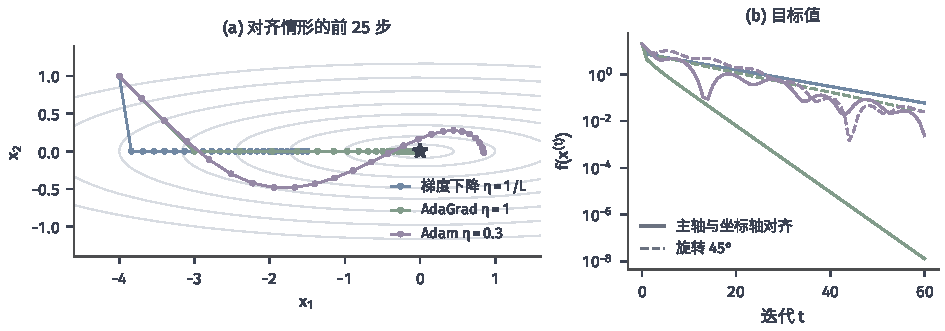
\includegraphics[width=160mm]{figures/03-optimization-evolution-and-signals/01-optimization/matplotlib/c6-adaptive-paths/figure.pdf}
  \caption{逐坐标缩放与坐标系的关系。目标$f(\bm x)=\tfrac12\bm x^\top\bm H\bm x$，精确梯度，初值$(-4,1)$。蓝：梯度下降，步长$1/L=1/25$；绿：AdaGrad，$\eta=1$；紫：Adam，$\eta=0.3$，$\beta_1=0.9$，$\beta_2=0.999$。(a) $\bm H=\operatorname{diag}(1,25)$时前$25$步的路径，灰色为等高线。(b) 目标值：实线为$\bm H=\operatorname{diag}(1,25)$，虚线为把$\bm H$与初值一起旋转$45^\circ$后的同一问题。梯度下降对旋转不变，两条蓝线重合。}
  \label{fig:opt-sto-adaptive-paths}
\end{figure*}

\subsection{Adafactor与统计压缩（补充）}
\label{sec:opt-sto-adafactor}

\paragraph{行列边际代替完整统计表}
神经网络的参数常以矩阵出现。对$\bm W\in\mathbb R^{m\times d}$，Adam式的平方统计$\bm V$与参数同形，要存$md$个数。Adafactor只保存它的行和$\bm R=\bm V\bm 1_d\in\mathbb R^m$与列和$\bm C=\bm V^\top\bm 1_m\in\mathbb R^d$，需要时用
\begin{equation}
\label{eq:opt-sto-adafactor}
  \hat{\bm V}=\frac{\bm R\bm C^\top}{\bm 1_m^\top\bm R}
\end{equation}
重建，存储从$O(md)$降到$O(m+d)$\scite{shazeer2018adafactor}。实际算法对$\bm G\odot\bm G+\epsilon_1$的行列和分别作指数平均，$\epsilon_1>0$保证重建的分母为正；然后用$\bm G/\sqrt{\hat{\bm V}}$作方向，并对这个方向按均方根裁剪、乘以与参数尺度成比例的相对步长。

\paragraph{压缩保留了什么}
式~\eqref{eq:opt-sto-adafactor}的重建保持行和与列和：$\hat{\bm V}\bm 1=\bm R\,(\bm C^\top\bm 1)/(\bm 1^\top\bm R)=\bm R$，列和同理。它丢失的是行列之间的交互。若$\bm V$的元素全为正，则$\hat{\bm V}=\bm V$当且仅当$\bm V$秩为一：若$\bm V=\bm u\bm w^\top$，则$\bm R=\bm u\,(\bm 1^\top\bm w)$、$\bm C=\bm w\,(\bm 1^\top\bm u)$，代入即得$\bm u\bm w^\top$；反之$\hat{\bm V}$按构造是秩一矩阵。例如$\bm V=\begin{bmatrix}1&2\\3&6\end{bmatrix}$可以精确恢复，而$\bm V=\begin{bmatrix}4&1\\1&4\end{bmatrix}$的行和、列和都是$(5,5)$，重建为全部元素等于$2.5$的矩阵，对角线上的大值与非对角的小值被抹平。图~\ref{fig:opt-sto-adafactor}在一个$6\times8$的例子上展示了这种误差：大尺度的行列结构被保留，个别元素的相对误差可达约$0.6$。

\begin{figure*}[!htbp]
  \centering
  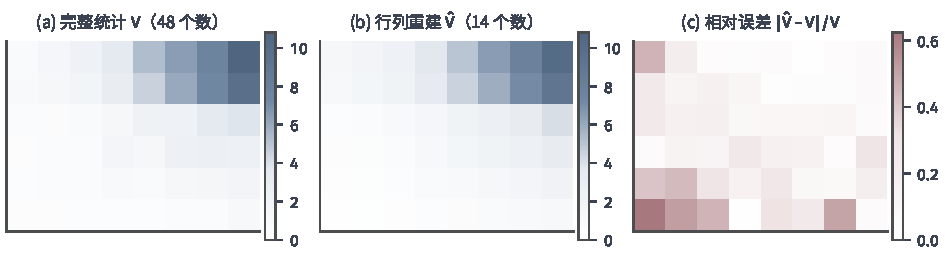
\includegraphics[width=160mm]{figures/03-optimization-evolution-and-signals/01-optimization/matplotlib/c6-adafactor/figure.pdf}
  \caption{平方统计的行列压缩。$40$个随机读数$\bm G_t=(\bm r\odot\bm z_t)\bm c^\top+0.6\bm E_t$，$\bm r$由$2$线性降到$0.5$，$\bm c$由$0.4$线性升到$1.6$，$\bm z_t$与$\bm E_t$为标准正态。(a) 逐元素平方的平均$\bm V$；(b) 由$6$个行和与$8$个列和按式~\eqref{eq:opt-sto-adafactor}重建的$\hat{\bm V}$；(c) 逐元素相对误差，平均约$0.18$，最大约$0.63$。}
  \label{fig:opt-sto-adafactor}
\end{figure*}

近似统计进入实际方向后，方向也随之改变：同一行内各列的相对缩放只由列和决定，无法表达“这一行的第$3$列特别大”。存储的减少与目标下降或收敛速度是两件事，需要分别评价；参数本身、读数和方向的计算仍是$O(md)$，低历史存储也不意味着整次训练的总成本更低。

\subsection{Shampoo与矩阵尺度（补充）}
\label{sec:opt-sto-shampoo}

\paragraph{两侧Gram统计}
逐坐标尺度把矩阵参数的每个元素看成独立的坐标，无法描述“某几行一起变化”这种方向关系。Shampoo为矩阵参数$\bm W\in\mathbb R^{m\times d}$维护左右两个Gram统计\scite{gupta2018shampoo}。取$\epsilon>0$，$\bm L^{(0)}=\epsilon\bm I_m$、$\bm R^{(0)}=\epsilon\bm I_d$，读取同一点的梯度矩阵$\bm G^{(t)}$后先更新统计，再变换方向：
\[
  \begin{gathered}
    \bm L^{(t+1)}=\bm L^{(t)}+\bm G^{(t)}\bm G^{(t)\top},\qquad
    \bm R^{(t+1)}=\bm R^{(t)}+\bm G^{(t)\top}\bm G^{(t)},\\
    \bm W^{(t+1)}=\bm W^{(t)}-\eta\,(\bm L^{(t+1)})^{-1/4}\bm G^{(t)}(\bm R^{(t+1)})^{-1/4}.
  \end{gathered}
\]
两个统计正定，负四分之一次幂由正交谱分解定义：若$\bm L=\bm Q\operatorname{diag}(\lambda_k)\bm Q^\top$，则$\bm L^{-1/4}=\bm Q\operatorname{diag}(\lambda_k^{-1/4})\bm Q^\top$。它们是梯度历史的矩阵函数，而不是目标的Hessian。

只看一步就能理解两侧四分之一次幂的作用。设$\epsilon\to0$，$\bm G$是方阵且可逆，奇异值分解为$\bm G=\bm U\bm\Sigma\bm V^\top$。则$\bm G\bm G^\top=\bm U\bm\Sigma^2\bm U^\top$，$\bm G^\top\bm G=\bm V\bm\Sigma^2\bm V^\top$，
\[
  (\bm G\bm G^\top)^{-1/4}\bm G(\bm G^\top\bm G)^{-1/4}=\bm U\bm\Sigma^{-1/2}\bm\Sigma\bm\Sigma^{-1/2}\bm V^\top=\bm U\bm V^\top ,
\]
所有奇异值被拉平为$1$，只保留奇异方向。例如$\bm G=\operatorname{diag}(4,1/4)$时，两侧的变换都是$\operatorname{diag}(1/2,2)$，方向变为单位矩阵：两个方向的幅度相差$16$倍，变换后相同。累积多步后，统计综合了历史上各方向的幅度，不再是这么干净的形式。

\paragraph{刷新频率与成本}
统计本身的存储为$O(m^2+d^2)$，形成$\bm G\bm G^\top$与$\bm G^\top\bm G$需要$O(m^2d+md^2)$，稠密谱分解求根一次约$O(m^3+d^3)$，应用两侧变换又是$O(m^2d+md^2)$。求根最贵，实际实现常每隔若干步才刷新一次矩阵根，中间沿用旧的根。这样本轮实际使用的尺度来自若干步之前的统计，与公式中的“先更新统计再用新统计”是不同的算法，记录实现时须写明刷新间隔。比较方法时，矩阵存储、分解、刷新和应用的成本都要计入，不能只比较参数更新次数。

\subsection{Lion符号动量法（补充）}
\label{sec:opt-sto-lion}

Lion只保留一个动量向量，并把方向的每个坐标取符号\scite{chen2023lion}。取$\bm m^{(0)}=\bm0$、$\beta_1,\beta_2\in[0,1)$、步长$\eta^{(t)}>0$与参数收缩系数$\lambda\geq0$，每轮依次执行
\[
  \begin{aligned}
    \bm z^{(t)}&=\beta_1\bm m^{(t)}+(1-\beta_1)\bm g^{(t)},\\
    \bm x^{(t+1)}&=\bm x^{(t)}-\eta^{(t)}\bigl(\operatorname{sign}(\bm z^{(t)})+\lambda\bm x^{(t)}\bigr),\\
    \bm m^{(t+1)}&=\beta_2\bm m^{(t)}+(1-\beta_2)\bm g^{(t)},
  \end{aligned}
\]
约定$\operatorname{sign}(0)=0$。构造方向用旧动量$\bm m^{(t)}$与系数$\beta_1$，更新状态用另一个系数$\beta_2$；如果先用$\beta_2$覆盖动量再算方向，就成了另一种算法。

符号运算保留每个坐标的方向，舍弃所有幅度。图~\ref{fig:opt-sto-lion-muon}(a)中，取$\bm m=\bm0$，读数$\bm g_{\mathrm a}=(0.2,0.05)$与$\bm g_{\mathrm b}=(4,1)$方向相同、长度相差$20$倍，Lion给出完全相同的方向$-(1,1)$；方向相近的$\bm g_{\mathrm c}=(3,-0.4)$却因第二坐标符号不同而给出$-(1,-1)$。不计收缩时，若方向有$q$个非零坐标，位移的欧氏范数恰为$\eta^{(t)}\sqrt q$，与读数大小无关。所以Lion的步长与梯度下降或Adam的步长数值不可比，它也不是对原目标的标准梯度步：即使读数是精确梯度，$\operatorname{sign}(\nabla f)$在最小点附近也不会变小，常数步长下迭代会在最小点附近以$\eta$的尺度来回跳动。是否在原目标上取得进展，仍要单独核验目标值或梯度残差。

\subsection{Muon矩阵动量法（补充）}
\label{sec:opt-sto-muon}

\paragraph{用极因子整形动量}
Muon同样处理矩阵参数，但不维护跨步的Gram统计，而是对当步的动量矩阵整形\scite{jordan2024muon}。动量取$\bm M^{(t+1)}=\beta\bm M^{(t)}+\bm G^{(t)}$（Nesterov形式改用$\bm G^{(t)}+\beta\bm M^{(t+1)}$作为待整形的矩阵）。设待整形矩阵$\bm H$的紧奇异值分解为$\bm H=\bm U_r\bm\Sigma_r\bm V_r^\top$，理想的整形输出是\term{极分解}（polar decomposition）中的因子$\bm O=\bm U_r\bm V_r^\top$：保留奇异方向，把所有正奇异值变为$1$。上一小节看到，单步的Shampoo变换给出同一个结果；Muon不累积历史，直接对当步动量求这个因子。

\paragraph{有限次矩阵迭代}
精确的奇异值分解太贵，Muon用矩阵多项式迭代近似极因子。先归一化$\bm X_0=\bm H/\lVert\bm H\rVert_F$，使所有奇异值落在$(0,1]$；再取$(a,b,c)=(3.4445,-4.7750,2.0315)$，执行$5$次
\[
  \bm A_k=\bm X_k\bm X_k^\top,\qquad\bm X_{k+1}=a\bm X_k+(b\bm A_k+c\bm A_k^2)\bm X_k .
\]
每次迭代保持奇异向量不变，把每个奇异值$s$映成$as+bs^3+cs^5$。最后取$\bm W^{(t+1)}=\bm W^{(t)}-\eta\,\gamma_{m,d}\bm X_5$，$\gamma_{m,d}$是依矩阵形状设定的尺度因子，原实现取$\sqrt{\max(1,m/d)}$。图~\ref{fig:opt-sto-lion-muon}(b)画出复合$5$次后的奇异值映射：对$s\in[0.02,1]$，输出落在约$[0.68,1.13]$内来回摆动，而不是精确的$1$。这组系数为了让小奇异值尽快抬升而牺牲了精度；作为对照，经典的三次Newton--Schulz迭代$\bm X_{k+1}=\tfrac32\bm X_k-\tfrac12\bm X_k\bm X_k^\top\bm X_k$在$s\in(0,1)$上单调逼近$1$，但$5$次后$s=0.01$只被抬到约$0.076$。

\begin{figure*}[!htbp]
  \centering
  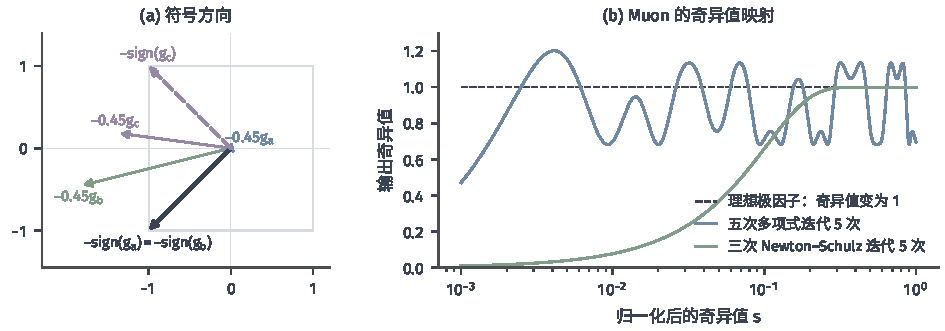
\includegraphics[width=160mm]{figures/03-optimization-evolution-and-signals/01-optimization/matplotlib/c6-lion-muon/figure.pdf}
  \caption{符号方向与奇异值整形。(a) Lion在$\bm m=\bm0$时的方向：细箭头为读数的相反方向$-0.45\bm g$，$\bm g_{\mathrm a}=(0.2,0.05)$、$\bm g_{\mathrm b}=(4,1)$、$\bm g_{\mathrm c}=(3,-0.4)$；粗箭头为$-\operatorname{sign}(\bm g)$，前两者相同，第三个不同。(b) 归一化奇异值$s$经$5$次迭代后的值，横轴为对数坐标：黑色虚线为理想极因子，蓝线为Muon的五次多项式$(a,b,c)=(3.4445,-4.7750,2.0315)$，绿线为三次Newton--Schulz迭代。}
  \label{fig:opt-sto-lion-muon}
\end{figure*}

\paragraph{近似、稳定处理与成本}
因此，实际算法的定义必须包括归一化方式、多项式系数、迭代次数、计算精度以及尺度因子；理想极因子的性质不能直接当作实际输出的性质。$\bm H$的某些奇异值极小时，归一化后的$s$可能低于多项式能有效抬升的范围，对应方向几乎不被放大。每次迭代需要三次矩阵乘法，代价约$O(md\min(m,d))$，$5$次迭代要计入每轮成本。矩阵方向的整形只用到当步动量，不涉及目标的二阶曲率。把参数更新与模型输出分布的几何联系起来的自然梯度、Fisher信息与K-FAC，属于分布几何的内容，可参考\BookChapterRef{chap:information-theory-and-statistical-geometry}{卷四“概率分布的分析与优化”章}。

\section{变量分块与交替优化}
\label{sec:opt-sto-block}

前面几节都在节省读取：每步读得少，但更新全部坐标。本节转到图~\ref{fig:opt-sto-sum-vs-block}的右半边，每轮只改变一部分变量。这样做的理由有两种：一部分变量的子问题可能便宜得多，甚至有闭式解；或者变量本身分成性质不同的几组，例如矩阵分解中的两个因子。问题在于，各块分别得到的改善能否拼成整体的改善，以及变量之间的耦合会留下什么困难。

\subsection{块梯度与块邻近更新}
\label{sec:opt-sto-block-gradient}

\paragraph{块光滑常数}
把坐标$\{1,\dots,d\}$划分为互不相交的块$J_1,\dots,J_B$，记$\bm x_J$为$\bm x$在块$J$上的分量，$\nabla_Jf(\bm x)$为对应的偏梯度，$\bm U_J\bm h$表示把$\bm h\in\mathbb R^{|J|}$放回块$J$、其余坐标补零的向量。若只沿块$J$移动时梯度的变化满足
\[
  \lVert\nabla_Jf(\bm x+\bm U_J\bm h)-\nabla_Jf(\bm x)\rVert_2\leq L_J\lVert\bm h\rVert_2\quad\text{对一切}\ \bm x,\bm h,
\]
就称$f$关于块$J$是$L_J$光滑的。与下降引理的证明完全相同，沿块$J$有二次上界$f(\bm x+\bm U_J\bm h)\leq f(\bm x)+\langle\nabla_Jf(\bm x),\bm h\rangle+\tfrac{L_J}2\lVert\bm h\rVert_2^2$。取$\bm h=-\nabla_Jf(\bm x)/L_J$，目标至少下降$\lVert\nabla_Jf(\bm x)\rVert_2^2/(2L_J)$。块光滑常数不超过整体的$L$，常常小得多：对最小二乘，单个坐标$j$的常数是$L_j=\lVert\bm A_{:,j}\rVert_2^2/n+\lambda$，即一个对角元，而$L$是整个矩阵的最大特征值。

\paragraph{计算单位}
一次块更新与一次完整循环是不同的计算单位。以最小二乘的单坐标更新为例，若维护残差$\bm r=\bm A\bm x-\bm b$，则$\partial_jf(\bm x)=\bm A_{:,j}^\top\bm r/n+\lambda x_j$只需$O(n)$，更新$x_j$后残差改变$\bm A_{:,j}\Delta x_j$，也是$O(n)$。遍历全部$d$个坐标一次的代价约为$O(nd)$，与一次梯度下降相当。因此比较坐标方法与梯度方法时，应以完整循环或总计算量为单位，而不是比较单步。

\paragraph{块邻近更新}
目标带有按块可分的非光滑项$F(\bm x)=f(\bm x)+\sum_kr_k(\bm x_{J_k})$时，把块梯度步换成块邻近梯度步：
\[
  \bm x_J\gets\operatorname{prox}_{r_J/L_J}\Bigl(\bm x_J-\frac1{L_J}\nabla_Jf(\bm x)\Bigr),
\]
其余块不变。它是第~\ref{chap:opt-nonsmooth}章邻近梯度法在单块上的版本。那里对凸的非光滑项、步长取光滑常数的倒数时证明了复合目标不增；把光滑常数换成块常数$L_J$，同一论证在单块上照样成立。$r_k=\lambda_1|\cdot|$的单坐标情形就是对最小二乘做软阈值，这是求解套索问题的常用方法。可分性在这里是本质的：非光滑项必须按块拆开，每块的邻近映射才能单独计算。

\paragraph{选块规则与新值的读取}
选块有三种常见规则。\emph{循环}规则按固定顺序依次更新，每块更新后立即用新值计算下一块的偏梯度。\emph{随机}规则每轮独立地均匀抽一块。\emph{贪心}规则选偏梯度最大的一块，需要维护全部偏梯度。另有一种并行做法让所有块都用上一轮的旧值同时更新，这实际上是一次带特殊步长的全梯度步，块上界不能保证它下降。对随机规则，每块的二次上界可以直接取期望。

\begin{theorem}[随机块坐标下降]
\label{thm:opt-sto-random-block}
设$f$关于每个块$J_k$是$L_{J_k}$光滑的，记$L_{\mathrm b}=\max_kL_{J_k}$，有下界$f^\star$。每轮与历史独立地均匀抽取一块$J$，令$\bm x_J\gets\bm x_J-\nabla_Jf(\bm x)/L_J$。则
\[
  \mathbb E_tf(\bm x^{(t+1)})\leq f(\bm x^{(t)})-\frac1{2B}\sum_{k=1}^B\frac{\lVert\nabla_{J_k}f(\bm x^{(t)})\rVert_2^2}{L_{J_k}}\leq f(\bm x^{(t)})-\frac{\lVert\nabla f(\bm x^{(t)})\rVert_2^2}{2BL_{\mathrm b}} .
\]
若$f$还是$\mu$强凸的，则$\mathbb Ef(\bm x^{(t)})-f^\star\leq\bigl(1-\mu/(BL_{\mathrm b})\bigr)^t\bigl(f(\bm x^{(0)})-f^\star\bigr)$。
\end{theorem}

\begin{proof}
抽到块$J_k$的概率为$1/B$，此时目标至少下降$\lVert\nabla_{J_k}f\rVert_2^2/(2L_{J_k})$，取平均即得第一个不等式；再用$L_{J_k}\leq L_{\mathrm b}$与$\sum_k\lVert\nabla_{J_k}f\rVert_2^2=\lVert\nabla f\rVert_2^2$。强凸时，对强凸下界$f(\bm y)\geq f(\bm x)+\langle\nabla f(\bm x),\bm y-\bm x\rangle+\tfrac\mu2\lVert\bm y-\bm x\rVert_2^2$两边对$\bm y$取最小值，得$f^\star\geq f(\bm x)-\lVert\nabla f(\bm x)\rVert_2^2/(2\mu)$，即$\lVert\nabla f(\bm x)\rVert_2^2\geq2\mu(f(\bm x)-f^\star)$。代入后减去$f^\star$、取全期望并反复使用即可。
\end{proof}

这个速率与随机抽样的随机梯度不同：读数没有噪声，只是每轮只走一个方向，所以收敛是线性的\scite{nesterov2012efficiency}。$B$次块更新大约等于一次完整循环，其收缩约为$(1-\mu/(BL_{\mathrm b}))^B\approx1-\mu/L_{\mathrm b}$；与梯度下降每步的$1-\mu/L$相比，块常数$L_{\mathrm b}$越小于$L$，坐标方法的优势越大。

\paragraph{阶梯路径与耦合}
图~\ref{fig:opt-sto-coordinate-descent}(a)在二次目标$\Phi(u,v)=\tfrac12(u-v)^2+\tfrac12(u-1)^2$上画出逐块精确最小化的循环坐标下降：路径只能沿坐标轴走，形成阶梯，在等高线细长且倾斜的方向上，每一阶都很短。精确地，固定$v$时最优$u=(v+1)/2$，固定$u$时最优$v=u$，所以每轮$v^{(t+1)}-1=\tfrac12(v^{(t)}-1)$，误差逐轮减半。变量间的耦合越强（等高线越斜越扁），阶梯越密，收敛越慢。

\begin{figure*}[!htbp]
  \centering
  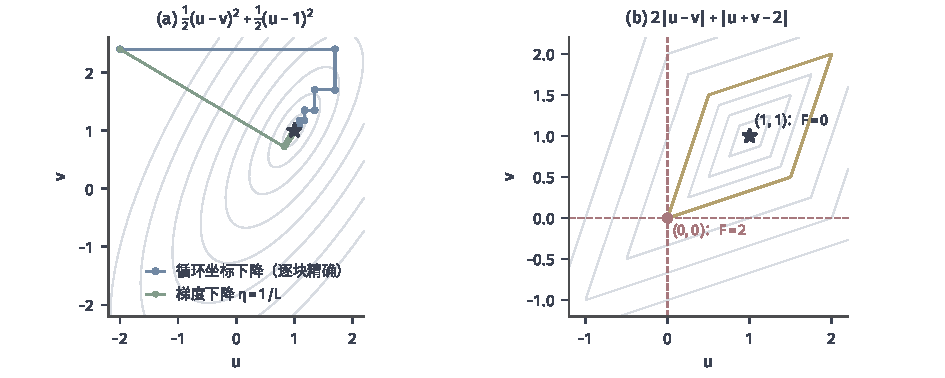
\includegraphics[width=160mm]{figures/03-optimization-evolution-and-signals/01-optimization/matplotlib/c6-coordinate-descent/figure.pdf}
  \caption{坐标下降的阶梯路径与停滞。(a) $\Phi(u,v)=\tfrac12(u-v)^2+\tfrac12(u-1)^2$，从$(-2,2.4)$出发：蓝线为循环坐标下降，每次精确最小化一个变量，$v$的误差逐轮减半；绿线为步长$1/L$的梯度下降。(b) 凸而不可分的非光滑目标$F(u,v)=2|u-v|+|u+v-2|$：在原点沿两条红色虚线方向，$F$都在原点取到唯一最小值$2$，坐标下降从原点出发永远不动；黄色为水平集$F=2$，真正的最小点是$(1,1)$，$F=0$。}
  \label{fig:opt-sto-coordinate-descent}
\end{figure*}

\paragraph{耦合约束与不可分非光滑项}
块方法的两类失败都来自耦合。第一类是约束把块绑在一起。若可行域是$\sum_jx_j=1$，从可行点出发只改一个坐标就会离开可行域，单坐标步要么不动、要么不可行；必须一次更新至少两个坐标，并让它们的变化相互抵消。第二类是非光滑项不可分。图~\ref{fig:opt-sto-coordinate-descent}(b)中$F(u,v)=2|u-v|+|u+v-2|$是凸函数，在原点$F=2$。固定$v=0$，$F(u,0)=2|u|+|u-2|$在$u<0$时斜率为$-3$，在$0<u<2$时斜率为$1$，所以$u=0$是唯一最小点；固定$u=0$同理。原点因此是每个坐标方向上的严格最小点，坐标下降在此永远停住，而$F(1,1)=0$。光滑时不会发生这种情况：各块偏梯度都为零就意味着整个梯度为零。

下降结论必须与实际规则匹配：循环、随机与贪心规则的保证各不相同，并行更新需要另外的步长条件；子问题若只近似求解，块上的下降量要扣除子问题误差，第~\ref{sec:opt-sto-perturbation}节会统一讨论这类误差。

\subsection{交替最小化}
\label{sec:opt-sto-alternating}

\paragraph{逐块求解条件子问题}
当某一块的子问题可以精确或高精度求解时，不必只走一步梯度，可以直接求出固定其余块后的最优解。对两块变量的目标$\Phi(\bm u,\bm v)$，\term{交替最小化}（alternating minimization）依次执行
\[
  \bm u^{(t+1)}\in\argmin_{\bm u}\Phi(\bm u,\bm v^{(t)}),\qquad
  \bm v^{(t+1)}\in\argmin_{\bm v}\Phi(\bm u^{(t+1)},\bm v).
\]
两步分别不增，连起来就是一轮改善：
\[
  \Phi(\bm u^{(t+1)},\bm v^{(t+1)})\leq\Phi(\bm u^{(t+1)},\bm v^{(t)})\leq\Phi(\bm u^{(t)},\bm v^{(t)}).
\]
条件子问题的最小点可能不唯一，这时算法必须事先规定\emph{平局规则}，例如“若当前值已是最小点之一就保持不变”，否则迭代序列没有明确定义。若子问题只近似求解，只要每块的返回值不比当前值差，单调性仍然成立；更细的精度要求留到误差分析。

\paragraph{分别凸不等于联合凸}
交替最小化常用于“固定一块后是凸问题”的目标，例如矩阵分解$\lVert\bm Y-\bm U\bm V^\top\rVert_F^2$：固定$\bm V$是关于$\bm U$的最小二乘，反之亦然。但分别凸并不保证联合凸，逐块精确也不保证达到全局最优。最小的例子是$\Phi(u,v)=\tfrac12(uv-1)^2$，它对$u$、对$v$分别是凸二次函数。从$(0,0)$出发，固定$v=0$时$\Phi(u,0)=\tfrac12$与$u$无关，每个$u$都是最小点，按“保持不变”的平局规则停在$u=0$；固定$u=0$同理。算法停在目标值$\tfrac12$，而全局最小值是$0$，在双曲线$uv=1$上取得。

加入正则项能消除平局，却消除不了停滞。$\Phi_\rho(u,v)=\tfrac12(uv-1)^2+\tfrac\rho2(u^2+v^2)$，$0<\rho<1$，条件子问题有唯一解$u=v/(v^2+\rho)$与$v=u/(u^2+\rho)$。从$(0,0)$出发，两式都给出$0$，算法仍停在原点；原点是驻点，其Hessian$\begin{bmatrix}\rho&-1\\-1&\rho\end{bmatrix}$有负特征值$\rho-1$，是一个鞍点。图~\ref{fig:opt-sto-alternating}取$\rho=0.05$：从$(3,0.1)$出发，路径沿弯曲的谷底以阶梯形逼近最小点$u=v=\sqrt{1-\rho}\approx0.975$，目标值从约$0.470$降到$8$轮后的约$0.0499$，最小值是$\rho-\rho^2/2=0.04875$；越靠近谷底，每一阶越短，这正是耦合造成的慢收敛；从原点出发则一步也不动，目标值停在$0.5$。

\begin{figure}[!htbp]
  \centering
  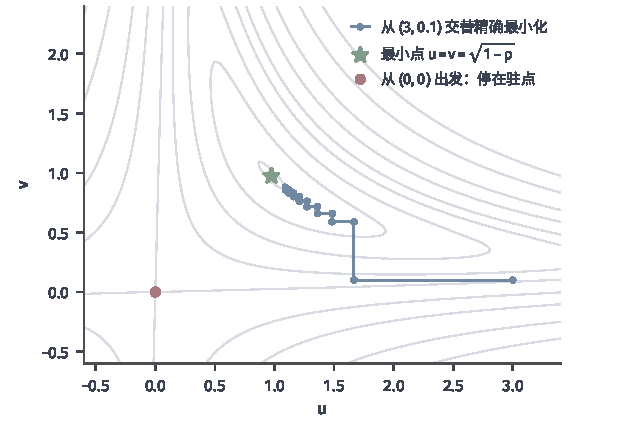
\includegraphics[width=105mm]{figures/03-optimization-evolution-and-signals/01-optimization/matplotlib/c6-alternating/figure.pdf}
  \caption{双线性目标上的交替最小化。$\Phi_\rho(u,v)=\tfrac12(uv-1)^2+\tfrac\rho2(u^2+v^2)$，$\rho=0.05$，灰色为等高线。蓝色阶梯从$(3,0.1)$出发，交替取$u=v/(v^2+\rho)$与$v=u/(u^2+\rho)$，画出前$8$轮，逐步逼近绿色星号处的最小点$u=v=\sqrt{1-\rho}$（另一最小点$u=v=-\sqrt{1-\rho}$未画出）。红点为原点：两个条件子问题的唯一解都是$0$，迭代停在这个鞍点。}
  \label{fig:opt-sto-alternating}
\end{figure}

\paragraph{能保证什么}
交替最小化的结论需要分层陈述。第一层是目标值单调不增，只要求每块返回不比当前更差的点；目标有下界时目标值序列收敛，但这并不说明迭代点收敛。第二层是聚点的块最优性：在目标连续、各条件子问题有唯一解等条件下，迭代序列的聚点在每一块上都是条件最优的；若目标还连续可微且无约束，各块偏梯度为零合起来就是整体驻点。图~\ref{fig:opt-sto-coordinate-descent}(b)说明非光滑不可分时这一步会失败。第三层是全局最优：联合凸时驻点就是全局最小点；不联合凸时，如上面的原点所示，驻点可能是鞍点。第四层是整个序列收敛到一点，这需要更强的条件，例如强凸性。期望最大化算法等具体统计方法也具有“交替求解条件子问题”的结构，在相应的概率模型建立之后，会复用这里的单调性论证，并同样面对停在非全局点的问题。

\section{方向信息的处理}
\label{sec:opt-sto-direction}

到目前为止，算法实际使用的方向要么是读数本身，要么是读数经过平均或缩放的结果。实践中还有两类更直接的改动：把过大的读数截短，以及在导数没有用处的地方人为指定一个反向传播规则。两者都会让实际方向偏离原目标的梯度。本节先给出操作的定义，再回到原目标检查所得方向的含义：计算图返回了一个向量，并不意味着这个向量是原目标的梯度，也不意味着沿它走一步会下降。

\subsection{梯度裁剪}
\label{sec:opt-sto-clipping}

\paragraph{两种裁剪}
\term{梯度裁剪}（gradient clipping）在读数过大时把它缩短，常用来防止个别巨大读数把参数推得太远，例如循环网络训练中梯度突然爆炸的情形\scite{pascanu2013}。给定阈值$c>0$，有两种做法。逐坐标裁剪把每个坐标截到区间$[-c,c]$内：
\[
  [\operatorname{clip}^{\mathrm{elem}}_c(\bm g)]_k=\max\{-c,\min\{c,g_k\}\};
\]
范数裁剪则整体缩放，只在范数超过阈值时生效：
\[
  \operatorname{clip}_c(\bm g)=\bm g\cdot\min\Bigl\{1,\frac{c}{\lVert\bm g\rVert_2}\Bigr\}.
\]
图~\ref{fig:opt-sto-clipping}(a)对同一个读数$\bm g=(3,4)$、$c=1$比较两者。逐坐标裁剪得到$(1,1)$，范数为$\sqrt2$，方向从与第一坐标轴夹角约$53^\circ$变成$45^\circ$；范数裁剪得到$(0.6,0.8)$，范数为$1$，方向不变。前者把读数投影到边长为$2c$的正方形上，后者投影到半径为$c$的圆盘上。

\paragraph{裁剪的位置}
裁剪放在算法的哪一环，得到的是不同的算法。裁剪原始读数，后续的动量和平方统计看到的是裁过的读数；裁剪经过统计缩放后的方向（Adafactor按均方根裁剪就是这一种），统计仍记录原始读数；裁剪最终位移，则限制的是$\lVert\bm x^{(t+1)}-\bm x^{(t)}\rVert_2$本身。在小批量中，先裁剪每个样本的读数再平均，与先平均再裁剪也不同。描述一个训练过程时必须写明裁剪的对象和阈值。

\paragraph{裁剪带来的偏差}
裁剪是非线性运算，它改变读数的平均。设标量读数以相等概率取$2$与$-1$，均值为$1/2$。用$c=1$裁剪后，读数变为$1$与$-1$，均值为$0$：期望方向消失了。图~\ref{fig:opt-sto-clipping}(b)画出裁剪后均值随阈值的变化：对这个两点分布，$c<1$时均值为$0$，$1\leq c<2$时为$(c-1)/2$，$c\geq2$时恢复为$1/2$；对向一侧拖尾的连续分布$-1+\operatorname{Exp}(1.5)$，均值随$c$平滑上升，但在任何有限阈值下都低于$1/2$。偏差的方向取决于读数分布的形状，不一定指向零。用第~\ref{sec:opt-sto-unbiased}节的分解，裁剪后的读数有非零的条件偏差$\bm\beta^{(t)}$，必须作为偏差处理，不能当作无偏梯度套用前面的定理。

\begin{figure*}[!htbp]
  \centering
  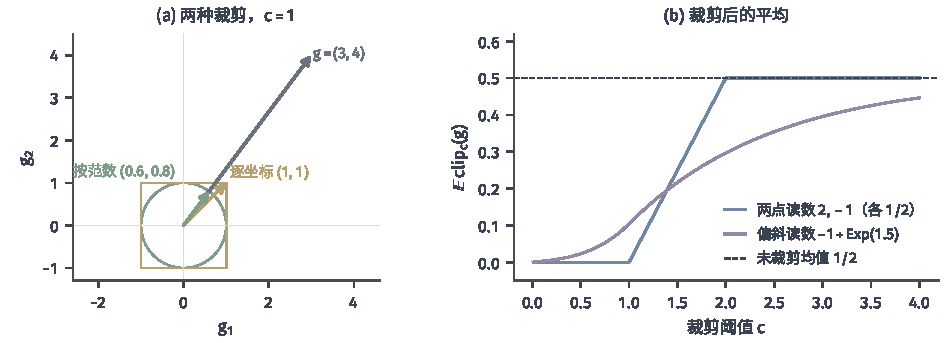
\includegraphics[width=160mm]{figures/03-optimization-evolution-and-signals/01-optimization/matplotlib/c6-clipping/figure.pdf}
  \caption{梯度裁剪的几何与偏差。(a) 读数$\bm g=(3,4)$，阈值$c=1$：逐坐标裁剪落在黄色正方形的角上，得到$(1,1)$；范数裁剪沿原方向缩到绿色单位圆上，得到$(0.6,0.8)$。(b) 标量读数裁剪后的均值$\mathbb E\operatorname{clip}_c(g)$随阈值$c$的变化。蓝线：以相等概率取$2$与$-1$；紫线：$g=-1+E$，$E$服从均值为$1.5$的指数分布。两者未裁剪时均值都是$1/2$（虚线）。}
  \label{fig:opt-sto-clipping}
\end{figure*}

增大批量能否减小这一偏差，取决于裁剪的位置。若逐样本裁剪后再平均，批量平均的是裁过的读数，期望仍是裁剪后的均值，偏差不随批量变小。若先平均再裁剪，批量越大，平均读数越集中在真梯度附近，被裁剪的概率越小；只要真梯度的范数小于阈值，偏差随批量增大而减小。

\paragraph{分别评价三种作用}
裁剪的作用应拆开评价。第一是限制位移：范数裁剪保证每步位移不超过$\eta c$，这是确定的。第二是引入偏差：如上所述，它使期望方向偏离梯度，在误差界中表现为不随步长消失的项，第~\ref{sec:opt-sto-perturbation}节会给出这一项的位置。第三是可能控制噪声：读数分布有重尾、二阶矩很大甚至无穷时，裁剪后的读数二阶矩有界，前面依赖方差假设的分析才有可能使用。是否值得用偏差换取有界的二阶矩，要看具体分布，不存在无条件的结论。

\subsection{离散前向与替代梯度（补充）}
\label{sec:opt-sto-surrogate}

\paragraph{导数处处为零的前向}
量化网络把连续参数取整后再使用。设$Q(w)=\operatorname{round}(w)$，损失$F(w)=\tfrac12(Q(w)-a)^2$。$Q$在非半整数点处局部为常数，所以除了可数个跳跃点外$F'(w)=0$：经典梯度不提供任何关于往哪边走的信息，梯度下降一步也不会动。这与第~\ref{sec:opt-sto-expectation}节的指示函数例同源：前向函数分片常数，信息全部藏在跳跃里。

\paragraph{直通估计}
\term{直通估计}（straight-through estimator）在反向计算时假装$Q$是恒等映射，即人为规定$\mathrm dQ/\mathrm dw=1$\scite{math-bengio2013estimating}，于是返回的方向是$g_{\mathrm{STE}}(w)=Q(w)-a$。这类人为指定的反向信号统称\term{替代梯度}（surrogate gradient）。区分两件事很重要：前向函数$F$是实际被评价的对象，反向规则是我们另外选的方向生成方式，两者之间没有求导关系。用有限差分检查得到的是前向函数的导数（这里是零），不能用来“验证”替代梯度。

图~\ref{fig:opt-sto-ste}给出同一点出发的两个结果。取$w=0.2$，$Q(w)=0$。若$a=1$，$F=0.5$，替代梯度为$-1$；取步长$0.4$走到$w=0.6$，$Q=1$，损失降为$0$。若$a=0.4$，$F=0.08$，替代梯度为$-0.4$；取步长$1$同样走到$w=0.6$，损失却升到$0.18$：$Q$跳过了目标$0.4$，落在另一侧更远的整数上。光滑下降的证明依赖于“小步之内一阶模型准确”，而跨过跳跃点时一阶模型完全失效，因此无法从替代梯度推出下降。

\begin{figure}[!htbp]
  \centering
  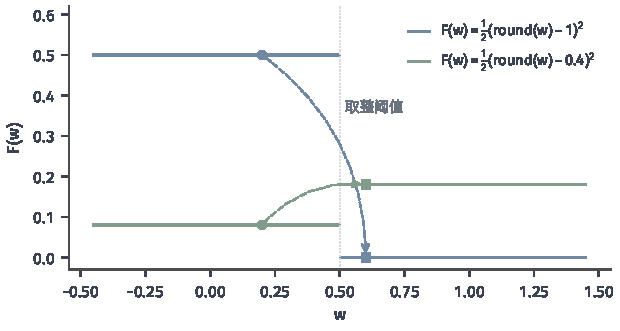
\includegraphics[width=105mm]{figures/03-optimization-evolution-and-signals/01-optimization/matplotlib/c6-ste/figure.pdf}
  \caption{取整前向上的直通估计。蓝线$F(w)=\tfrac12(\operatorname{round}(w)-1)^2$，绿线$F(w)=\tfrac12(\operatorname{round}(w)-0.4)^2$，两者都是分段常数，经典导数几乎处处为零；点线为取整阈值$w=0.5$。圆点为起点$w=0.2$，方块为沿替代梯度$\operatorname{round}(w)-a$走一步后的位置$w=0.6$：蓝色（步长$0.4$）损失由$0.5$降到$0$，绿色（步长$1$）损失由$0.08$升到$0.18$。}
  \label{fig:opt-sto-ste}
\end{figure}

\paragraph{替代方向的地位}
替代梯度一般既不是经典梯度，也不是次梯度。以$a=1$、$w=0.2$为例：要求$F(y)\geq F(w)+s(y-w)$对一切$y$成立的斜率$s$并不存在，因为$y=0.6$处要求$s\leq-1.25$，$y=-0.4$处（$F$仍为$0.5$）要求$s\geq0$；只看局部时$F$在该点附近为常数，局部意义下的次梯度只有$0$。替代梯度$-1$两者都不是。所以训练是否成功只能回到实际的前向任务上评价：比较前向损失、验证指标或原问题的目标值，而不是看替代梯度的范数是否变小。停止准则也应基于前向量。

\paragraph{向量量化与停止梯度}
\term{向量量化}（vector quantization）把编码器输出$\bm z$替换为码本中最近的向量$\bm e_{k^\star}$，$k^\star=\argmin_k\lVert\bm z-\bm e_k\rVert_2$，选择最近者也是分段常数的运算。常见做法用一个\term{停止梯度}（stop-gradient）标记$\operatorname{sg}$写成$\bm z_q=\bm z+\operatorname{sg}(\bm e_{k^\star}-\bm z)$\scite{nlp-speech-oord2017vqvae}：前向时$\operatorname{sg}$原样传值，所以$\bm z_q=\bm e_{k^\star}$；反向时$\operatorname{sg}$阻断传播，所以对$\bm z$的反向信号相当于单位Jacobian，编码器得到的是直通方向。码本向量本身收不到这条路径的信号，必须另行规定更新，例如在损失中加入$\lVert\operatorname{sg}(\bm z)-\bm e_{k^\star}\rVert_2^2$，或用编码器输出的移动平均更新码本。需要注意，$\operatorname{sg}$是计算图上的传播规则，不是一个普通函数：不存在一个函数既处处等于恒等映射又导数为零。把它当作函数去求导或分析，会得到自相矛盾的结论。

\section{算法的扰动分析}
\label{sec:opt-sto-perturbation}

前面各节分别遇到了几种与理想梯度的偏离：零均值的噪声、裁剪造成的偏差、近似求解的子问题。本节把它们放在一起，问一个共同的问题：固定一个运行有限步的算法，改变它的输入，输出会变多少。输入的改变有两种。一种是方向读数被扰动，数据不变；另一种是数据集中换掉一个样本，算法规则不变。研究对象是“算法映射”，即从数据和随机下标路径到返回点的映射，这与第~\ref{chap:opt-smooth}章研究问题参数变化时\emph{精确}最优解如何移动的敏感性分析不同：那里不涉及算法跑了几步，这里不涉及精确解。

\subsection{读数误差与原目标进展}
\label{sec:opt-sto-reading-error}

\paragraph{三种误差进入递推的位置}
在同一个数据集上，实际方向与真梯度的差可以分成三类。条件噪声$\bm\xi^{(t)}$满足$\mathbb E_t\bm\xi^{(t)}=\bm0$，来自随机抽样。系统偏差$\bm\beta^{(t)}$由历史决定，来自裁剪、量化、过时的参数或有偏的抽样。子问题误差来自块更新、邻近映射或交替最小化中没有精确求解的子问题，若以返回点与精确子问题解的差来计，它也是一个由当前状态决定的偏差。第~\ref{chap:opt-smooth}章已经用这种拆分分析过不精确梯度的梯度下降；这里只把条件期望加进去。

把$\bm g^{(t)}=\nabla f(\bm x^{(t)})+\bm\beta^{(t)}+\bm\xi^{(t)}$代入下降引理，取$\mathbb E_t$。设$\lVert\bm\beta^{(t)}\rVert_2\leq B$，$\mathbb E_t\lVert\bm\xi^{(t)}\rVert_2^2\leq\sigma^2$，$\eta\leq1/L$。记$\bm a=\nabla f(\bm x^{(t)})$，由$-\eta\langle\bm a,\bm a+\bm\beta\rangle+\tfrac\eta2\lVert\bm a+\bm\beta\rVert_2^2=\tfrac\eta2(\lVert\bm\beta\rVert_2^2-\lVert\bm a\rVert_2^2)$，得到
\begin{equation}
\label{eq:opt-sto-biased-step}
  \mathbb E_tf(\bm x^{(t+1)})\leq f(\bm x^{(t)})-\frac\eta2\lVert\nabla f(\bm x^{(t)})\rVert_2^2+\frac\eta2B^2+\frac{L\eta^2}2\sigma^2 .
\end{equation}
求和后与定理~\ref{thm:opt-sto-nonconvex}相同地处理，常数步长下
\[
  \frac1T\sum_{t<T}\mathbb E\lVert\nabla f(\bm x^{(t)})\rVert_2^2\leq\frac{2\bigl(f(\bm x^{(0)})-f_{\inf}\bigr)}{\eta T}+B^2+L\eta\sigma^2 .
\]
三项分别对应初始误差、偏差和噪声。初始误差项随$T$消失；噪声项正比于$\eta$，用小批量还会变成$L\eta\sigma^2/b$；偏差项$B^2$既不依赖$\eta$，也不依赖$T$和批量，是一个硬性的下限。

\paragraph{二次目标上的轨迹}
在二次目标$f(\bm x)=\tfrac12(\bm x-\bm x^\star)^\top\bm H(\bm x-\bm x^\star)$上，轨迹的差可以精确写出：
\[
  \bm x^{(t+1)}-\bm x^\star=(\bm I-\eta\bm H)(\bm x^{(t)}-\bm x^\star)-\eta\bm\beta-\eta\bm\xi^{(t)} .
\]
若偏差是常向量$\bm\beta$，期望迭代收敛到$\bm x^\star-\bm H^{-1}\bm\beta$：偏差把整条轨迹平移到一个新的不动点，平移量$\bm H^{-1}\bm\beta$与步长无关，并在小曲率方向被放大。噪声则在这个点附近造成与$\eta$成正比的波动。图~\ref{fig:opt-sto-perturbation}(a)在二维最小二乘上验证这一点：只有噪声时，误差平台随步长缩小为四分之一而缩小到约四分之一，用$4$个样本的批量效果相同；只有偏差时，两种步长最终停在同一个高度$\lVert\bm H^{-1}\bm\beta\rVert_2^2\approx0.023$，小步长只是到达得更慢。

\begin{figure*}[!htbp]
  \centering
  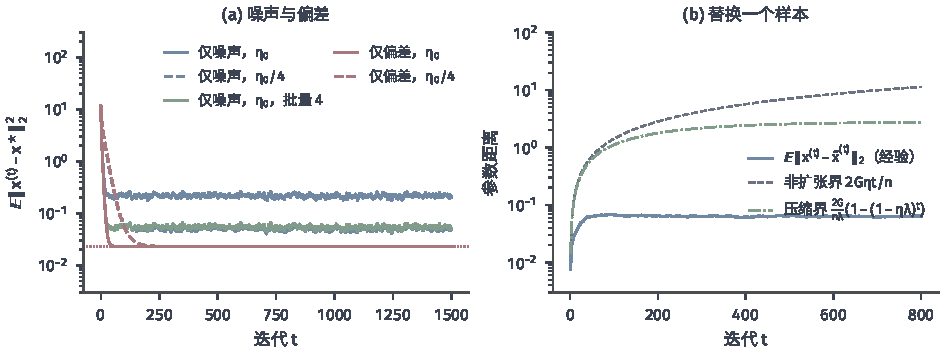
\includegraphics[width=160mm]{figures/03-optimization-evolution-and-signals/01-optimization/matplotlib/c6-perturbation/figure.pdf}
  \caption{两种输入扰动下的算法输出。问题同图~\ref{fig:opt-sto-noise-ball}。(a) 读数为$\nabla f(\bm x)+\bm\beta+\bm\xi/\sqrt b$：仅噪声时$\bm\beta=\bm0$、$\bm\xi\sim N(\bm0,0.25\bm I)$，仅偏差时$\bm\beta=(0.25,0)$、$\bm\xi=\bm0$；$\eta_0=0.4$，$300$次运行平均。红色点线为$\lVert\bm H^{-1}\bm\beta\rVert_2^2$。(b) 把第$1$个样本换成新样本后，以相同初值$\bm0$、相同下标路径和步长$1/L_{\max}$运行两份数据，$2000$次运行的平均参数距离（蓝），以及定理~\ref{thm:opt-sto-stability}的非扩张界与利用正则项强凸性的压缩界，纵轴为对数坐标。$G\approx2.78$是两条路径上被替换两项梯度范数的最大值。}
  \label{fig:opt-sto-perturbation}
\end{figure*}

\paragraph{哪种手段改善哪一项}
这个分解说明了常见调节手段各自作用于哪一项。增大批量或缩小步长只压低噪声项。去掉偏差需要改变读数本身：放宽裁剪阈值、使用无偏的抽样权重、使用更新的参数。子问题误差则要靠把子问题解得更准来减小，每一轮的子问题误差都像偏差一样进入递推。如果偏差项已经占主导，继续增大批量或延长运行都无济于事。

\paragraph{带历史的方法与不同的误差对象}
动量、Adam、SAGA这类方法的下一步不仅取决于当前参数，还取决于动量、统计量或梯度表。比较两次运行时，必须把完整状态作为比较对象：参数相同而动量不同，未来的轨迹也不同。另外要区分三种误差对象：目标误差邻域（期望目标差停在多高）、期望驻点残差（梯度范数平方的平均）以及实际轨迹的偏差（某次运行与参考轨迹的距离）。随机梯度运行中目标估计值的波动，很大部分来自评估目标所用的抽样，不直接等于参数不稳定；反过来，参数几乎不动也不说明已经接近最优，偏差项可能正把它固定在一个错误的位置。

\subsection{样本替换的有限步响应}
\label{sec:opt-sto-stability}

\paragraph{耦合两次运行}
现在固定读数规则，改变数据。设数据集$S$与$S'$只有第$k$个样本不同，对应的逐项函数为$f_i$与$f_i'$，$i\neq k$时$f_i=f_i'$。在两份数据上运行随机梯度下降，使用相同的初值、相同的步长和\emph{相同的}下标序列$i^{(0)},i^{(1)},\dots$，得到$\bm x^{(t)}$与$\tilde{\bm x}^{(t)}$。这种耦合把抽样噪声的影响去掉，两条轨迹的差只来自被替换的样本。

\paragraph{非扩张的梯度步}
没有抽到第$k$项时，两条轨迹用同一个函数$f_i$走一步。下面的性质说明这一步不会拉开距离。

\begin{lemma}[凸光滑函数梯度步的非扩张性]
\label{lem:opt-sto-nonexpansive}
设$\phi$凸且$L$光滑，$0\leq\eta\leq2/L$。则对任意$\bm x,\bm y$，$\lVert(\bm x-\eta\nabla\phi(\bm x))-(\bm y-\eta\nabla\phi(\bm y))\rVert_2\leq\lVert\bm x-\bm y\rVert_2$。
\end{lemma}

\begin{proof}
把引理~\ref{lem:opt-sto-cocoercive}分别用于$(\bm x,\bm y)$和$(\bm y,\bm x)$再相加，函数值项相消，得到$\lVert\bm\Delta\rVert_2^2\leq L\langle\bm\Delta,\bm x-\bm y\rangle$，其中$\bm\Delta=\nabla\phi(\bm x)-\nabla\phi(\bm y)$。于是
$\lVert\bm x-\bm y-\eta\bm\Delta\rVert_2^2=\lVert\bm x-\bm y\rVert_2^2-2\eta\langle\bm\Delta,\bm x-\bm y\rangle+\eta^2\lVert\bm\Delta\rVert_2^2\leq\lVert\bm x-\bm y\rVert_2^2-\eta(2/L-\eta)\lVert\bm\Delta\rVert_2^2$，当$\eta\leq2/L$时最后一项非正。
\end{proof}

\begin{theorem}[样本替换下的期望参数距离]
\label{thm:opt-sto-stability}
设每个$f_i$与$f_k'$凸且$L$光滑，下标独立均匀抽取，确定的步长满足$0\leq\eta^{(t)}\leq2/L$，并设在两条轨迹访问过的点上，被替换的两项梯度满足$\lVert\nabla f_k(\bm x^{(t)})\rVert_2\leq G$与$\lVert\nabla f_k'(\tilde{\bm x}^{(t)})\rVert_2\leq G$。则
\begin{equation}
\label{eq:opt-sto-stability}
  \mathbb E\lVert\bm x^{(T)}-\tilde{\bm x}^{(T)}\rVert_2\leq\frac{2G}{n}\sum_{t<T}\eta^{(t)} .
\end{equation}
\end{theorem}

\begin{proof}
记$\delta_t=\lVert\bm x^{(t)}-\tilde{\bm x}^{(t)}\rVert_2$，$\delta_0=0$。若$i^{(t)}\neq k$，两条轨迹对同一个$f_i$作梯度步，由引理~\ref{lem:opt-sto-nonexpansive}，$\delta_{t+1}\leq\delta_t$。若$i^{(t)}=k$，由三角不等式，$\delta_{t+1}\leq\delta_t+\eta^{(t)}\bigl(\lVert\nabla f_k(\bm x^{(t)})\rVert_2+\lVert\nabla f_k'(\tilde{\bm x}^{(t)})\rVert_2\bigr)\leq\delta_t+2\eta^{(t)}G$。下标与历史独立，后一种情形的条件概率为$1/n$，所以$\mathbb E_t\delta_{t+1}\leq\delta_t+2\eta^{(t)}G/n$。取全期望并累加即得。
\end{proof}

这个界的结构很直观：每一步以概率$1/n$注入至多$2\eta^{(t)}G$的差异，注入之后的差异不会被后续步骤放大。若每项还是$\lambda$强凸的且二阶连续可微，$\eta\leq2/(L+\lambda)$时梯度步的Jacobian$\bm I-\eta\nabla^2f_i$的特征值落在$[-(1-\eta\lambda),1-\eta\lambda]$内，非扩张可以加强为以因子$1-\eta\lambda$压缩，差异的递推变为$\mathbb E\delta_{t+1}\leq(1-\eta\lambda)\mathbb E\delta_t+2\eta G/n$，界不再随$T$无限增长，而是停在$2G/(n\lambda)$以下。图~\ref{fig:opt-sto-perturbation}(b)中，平均距离在约$50$步内升到约$0.06$后保持稳定；非扩张界随$t$线性增长，在$t=20$时已是实际值的约$7$倍，压缩界则趋于约$2.7$。两个界都正确但偏保守，原因是$G$取了路径上的最大值，而实际注入的差异多数时候远小于$2\eta G$。

\paragraph{这个界说明了什么，没有说明什么}
式~\eqref{eq:opt-sto-stability}描述的是运行有限步的算法映射对单个样本的敏感程度，属于\term{算法稳定性}（algorithmic stability）的一种形式\scite{hardt2016sgd}。它与固定目标下的抽样噪声是两回事：同一份数据、不同下标路径的两次运行，距离由噪声邻域决定，可能比这里的距离大得多；这里刻意用同一条下标路径把那部分去掉。条件也需要逐项核对：要求的是\emph{每一项}凸，而不只是平均目标凸；梯度界$G$只需在实际访问的点上对被替换的两项成立，对最小二乘这样梯度随参数增长的目标，它依赖于轨迹停留的区域。若要把参数距离转为损失之差，还需要损失对参数的Lipschitz常数$K$，得到$|\ell(\bm x^{(T)};z)-\ell(\tilde{\bm x}^{(T)};z)|\leq K\lVert\bm x^{(T)}-\tilde{\bm x}^{(T)}\rVert_2$。至于从这里推出关于未见数据的泛化结论，还需要统计论证，由后续讨论学习理论的部分承担。

\section{计算成本与方法比较}
\label{sec:opt-sto-cost}

本章的方法可以归为四类计算安排：减少每步读取（随机梯度、非均匀抽样、小批量），复用历史信息（SVRG、SAGA与各种自适应统计），限制每步更新的范围（坐标下降与交替最小化），以及改变方向本身（裁剪、符号、矩阵整形、替代梯度）。要比较它们，必须先让原目标、返回对象和精度要求一致，再用同一个预算口径计数。本节给出这个口径，并说明在什么情况下哪一项成本才是真正的瓶颈。

\paragraph{计数单位与登记项目}
四种单位常被混用：一次梯度读取（求一个$\nabla f_i$）、一次参数更新、一次全数据遍历（$n$次读取）和一次完整分块循环（每块各更新一次）。随机梯度一次更新读$1$项，梯度下降读$n$项，SVRG的外循环读$n+2m$项，块坐标下降的一次完整循环在最小二乘上约等于一次梯度的计算量。除读取之外，还要登记方法特有的成本：快照的完整梯度、梯度表与统计量的存储、矩阵求根与分解、子问题的求解以及抽样分布的维护。表~\ref{tab:opt-sto-costs}汇总本章各方法的这些项目。

\begin{table*}[!htbp]
  \centering
  \caption{本章方法的每步成本与本章给出的保证。$n$为项数，$d$为参数维数，矩阵参数为$m\times d$，$b$为批量，$m_{\mathrm{in}}$为SVRG内循环长度。“读取”按单项梯度计。保证一栏只列本章正文实际给出或引用的结论及其主要条件。}
  \label{tab:opt-sto-costs}
  \footnotesize
  \begin{tabularx}{\linewidth}{@{}l>{\raggedright\arraybackslash}p{24mm}>{\raggedright\arraybackslash}p{20mm}>{\raggedright\arraybackslash}p{26mm}>{\raggedright\arraybackslash}X@{}}
    \toprule
    方法 & 每次更新读取 & 额外状态 & 额外计算 & 本章的保证（主要条件）\\
    \midrule
    梯度下降 & $n$ & — & — & 对照基准（第~\ref{chap:opt-smooth}章）\\
    随机梯度 & $1$ & — & — & 噪声邻域、$1/t$与$1/\sqrt T$速率（无偏、矩条件）\\
    非均匀抽样 & $1$ & 分布$O(n)$ & 抽样$O(1)$至$O(\log n)$ & 同上，常数由$p$决定（反比权重）\\
    小批量 & $b$ & — & — & 噪声项除以$b$（批内条件独立）\\
    SVRG & $2$，每外循环另加$n$ & $O(d)$ & — & 外循环线性收敛（每项凸光滑、$f$强凸）\\
    SAGA & $1$，初始化$n$ & $O(nd)$梯度表 & — & 线性收敛（同上，引用）\\
    AdaGrad、RMSProp & $1$ & $O(d)$ & $O(d)$ & 依具体分析而定（引用）\\
    Adam、AMSGrad & $1$ & $O(2d)$ & $O(d)$ & 依具体分析而定（引用）\\
    Adafactor & $1$ & $O(m+d)$ & $O(md)$重建 & 存储压缩；收敛另需论证\\
    Shampoo & $1$ & $O(m^2+d^2)$ & 求根$O(m^3+d^3)$/刷新 & 凸在线分析（引用）\\
    Lion & $1$ & $O(d)$ & $O(d)$ & 无一般保证；位移长$\eta\sqrt q$\\
    Muon & $1$ & $O(md)$动量 & $5$次迭代$O(md\min(m,d))$ & 无一般保证\\
    随机块坐标 & 一块的偏梯度 & — & 维护残差 & 强凸时线性收敛（块光滑）\\
    交替最小化 & 子问题所需 & — & 子问题求解 & 目标单调；块最优（附加条件）\\
    \bottomrule
  \end{tabularx}
\end{table*}

\paragraph{先固定误差对象}
不同方法的结论针对不同的误差对象：期望目标差、到最小点的期望距离、梯度平方残差的平均，或者带证书的目标差上界。返回对象也不同：最后一点、加权平均点、随机返回点。比较时应先选定一个误差对象和一个返回规则，对每种方法计算达到同一精度的总成本，而不是比较每步成本，也不是比较外层迭代次数。SVRG的一个外循环和随机梯度的一步完全不可比；Shampoo的一次参数更新若带一次矩阵求根，也不能与Adam的一次更新等量齐观。

\paragraph{抽样误差何时成为主要限制}
由定理~\ref{thm:opt-sto-constant-step}，常数步长随机梯度的误差由两部分组成：随迭代几何衰减的初始误差，以及大小约为$2\eta\sigma_\star^2/(b\mu)$的噪声平台。若目标精度远高于平台，噪声就是主要限制，此时增大批量与缩小步长等价，都要付出更多读取；若目标精度低于平台，噪声并不是问题，限制来自曲率，增大批量只是浪费。图~\ref{fig:opt-sto-batch-cost}把这一点画成曲线：在$n=10000$的最小二乘上，对每个批量$b$取最优的常数步长，计算期望目标差首次达到$10^{-3}$所需的读取量。$b\leq64$时读取量几乎不变，约$4.1\times10^4$，批量增大$b$倍，所需步数也减少约$b$倍；$b$超过数百后，最优步长已增大到$1/L$附近并逼近稳定上限$2/L$，步数不能再按比例减少，读取量随之上升，$b=4096$时约为$1.4\times10^5$。梯度下降需要$4.3\times10^5$次读取。这条曲线中“平坦段”到“上升段”的转折，就是噪声主导与曲率主导的分界。

\begin{figure}[!htbp]
  \centering
  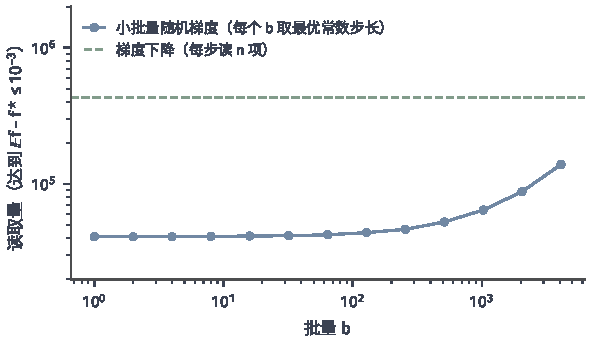
\includegraphics[width=100mm]{figures/03-optimization-evolution-and-signals/01-optimization/matplotlib/c6-batch-cost/figure.pdf}
  \caption{达到同一精度所需的读取量随批量的变化。岭回归最小二乘，$n=10000$，$d=5$，$\lambda=10^{-2}$，$L\approx1.00$，$\mu\approx0.050$，初值$\bm0$。蓝线：小批量随机梯度（有放回抽样），每个$b$在$80$个候选常数步长中取最优者，读取量指期望目标差首次不超过$10^{-3}$时已读取的样本数；期望由一阶与二阶矩的精确递推算出，没有蒙特卡罗误差。绿色虚线：步长$1/L$的梯度下降，$43$步、每步读$n$项。双对数坐标。}
  \label{fig:opt-sto-batch-cost}
\end{figure}

\paragraph{内层精度、批量与记忆的代价}
同样的推理适用于子问题。交替最小化或块邻近步骤中，如果子问题误差远小于外层每轮的改善，继续解准子问题没有意义；如果子问题误差与外层改善同量级，它就像偏差一样形成误差下限（第~\ref{sec:opt-sto-reading-error}节），此时解准内层才有回报。方差缩减与增大批量是两种降噪的代价形式：前者用$O(d)$的快照加周期性的全数据遍历，或用$O(nd)$的梯度表，换取线性收敛；后者用每步$b$倍的读取换取$1/b$的噪声。数据可以反复访问、$n$不太大时前者通常更省；数据流式到来或存储受限时，只能用后者。

\paragraph{比较时必须保持一致的约定}
最后，几个容易被忽略的约定会直接改变比较结果。目标是否除以$n$决定了光滑常数与梯度的量级，从而决定步长的数值，所以报告步长时要说明目标的归一化方式。停止准则要相同：一种方法按梯度范数停止，另一种按目标估计停止，二者不可比。返回对象要相同：用平均点评价一种方法、用最后一点评价另一种，会把返回规则的差异误当作方法的差异。在这些约定一致之后，读取、计算与存储的总量才是有意义的比较依据。

\section{本章小结}
\label{sec:opt-sto-summary}

章首的问题是：一百万行的最小二乘，若每步只读一行，单步方向可能指向上坡，许多步合起来是否仍在下降，又会停在哪里。本章的回答以有限步的期望误差为主线。只读一项的随机梯度只要在给定历史下条件无偏，代入光滑上界取条件期望后，期望下降与噪声上升就分成正比于$\eta$和$\eta^2$的两项。强凸时，常数步长使期望误差几何下降到一个与$\eta\sigma_\star^2/\mu$成正比的噪声邻域；递减步长$2/(\mu(t+t_0))$把它推向零，速率为$1/t$；凸目标的加权平均点和非凸目标的随机返回点分别有$1/\sqrt T$量级的界。这些界针对指定的返回对象，是期望意义下的结论；单条路径的几乎必然收敛属于随机逼近理论。

有限和、期望与变量分块三种结构分别支持三种节省。有限和允许只读一部分项，也允许反复访问同一项，因此可以用快照（SVRG）或逐项记忆（SAGA）把读数方差降到随迭代趋于零，在每项凸光滑、目标强凸时恢复线性收敛；期望目标只能不断抽取新样本，方差只能靠批量按$1/b$压低。非均匀抽样必须按抽样概率的倒数重加权才保持无偏，它可能改善步长上限，也可能增大噪声。历史读数还可以给出尺度：AdaGrad、RMSProp、Adam等逐坐标方法在问题的难点与坐标轴对齐时收益明显，旋转之后便失去优势；Adafactor压缩统计的存储，Shampoo与Muon在矩阵参数上处理行列方向，它们的成本和保证都必须连同各自的条件说明。变量分块的收益依赖于块常数小于整体光滑常数，失败来自耦合：耦合约束、不可分的非光滑项，以及分别凸而不联合凸的目标都可能让逐块精确的算法停在非最优点。

几个界限贯穿全章。条件偏差，无论来自裁剪、有偏抽样还是不精确的子问题，都在误差界中留下不随步长、批量和迭代次数消失的项；替代梯度连偏差都谈不上，只能回到实际前向任务上评价。算法的输出对单个样本替换的敏感程度可以在每项凸光滑的条件下用有限步界控制，但这不是泛化结论。最后，比较方法时要先固定目标的归一化、误差对象、返回点和停止准则，再统计读取、计算与存储的总量。长期过程的收敛归第~\ref{chap:stochastic-processes-and-approximation}章，数据误差与泛化由后续讨论学习理论的部分承担。

